\documentclass[11pt,a4paper]{article}

\usepackage[T1]{fontenc}
\usepackage[utf8]{inputenc}
\usepackage[provide=*,main=english]{babel}
\usepackage{lmodern}
\usepackage{microtype}
\usepackage{geometry}
\geometry{top=2.25cm,bottom=2.35cm,left=2.35cm,right=2.35cm}
\usepackage{amsmath,amssymb,amsthm,mathtools,bm}
\usepackage{graphicx}
\usepackage{booktabs,tabularx,array,multirow,longtable}
\usepackage{enumitem}
\usepackage{xcolor}
\usepackage{caption}
\usepackage{subcaption}
\usepackage{fancyhdr}
\usepackage{hyperref}
\usepackage[nameinlink,noabbrev]{cleveref}

\definecolor{deepblue}{RGB}{21,101,192}
\definecolor{deeporange}{RGB}{216,67,21}
\definecolor{deepgreen}{RGB}{46,125,50}
\definecolor{softblue}{RGB}{232,242,252}
\definecolor{softgray}{RGB}{246,247,249}
\hypersetup{
  colorlinks=true,
  linkcolor=deepblue,
  citecolor=deepblue,
  urlcolor=deeporange,
  pdftitle={Equilibria and recurrent dynamics of normalized Transformer blocks},
  pdfauthor={Anonymous submission}
}

\pagestyle{fancy}
\fancyhf{}
\fancyhead[L]{Spherical Transformer dynamics}
\fancyhead[R]{Equilibria, cycles, and chaos}
\fancyfoot[C]{\thepage}
\setlength{\headheight}{14.3pt}
\setlength{\parindent}{0pt}
\setlength{\parskip}{0.52em}
\setlength{\emergencystretch}{3em}
\setcounter{tocdepth}{1}
\setlist{nosep,leftmargin=*}

\newtheorem{theorem}{Theorem}[section]
\newtheorem{proposition}[theorem]{Proposition}
\newtheorem{lemma}[theorem]{Lemma}
\newtheorem{corollary}[theorem]{Corollary}
\theoremstyle{definition}
\newtheorem{definition}[theorem]{Definition}
\newtheorem{remark}[theorem]{Remark}

\newcommand{\sphere}{\mathbb S}
\newcommand{\R}{\mathbb R}
\newcommand{\T}{\mathsf T}
\newcommand{\e}{\mathrm e}
\newcommand{\norm}[1]{\left\lVert #1\right\rVert}
\newcommand{\one}{\bm 1}
\newcommand{\N}{\mathcal N}
\newcommand{\Pperp}[1]{P_{#1}^{\perp}}
\newcommand{\diag}{\operatorname{diag}}
\newcommand{\Diag}{\operatorname{Diag}}
\newcommand{\rank}{\operatorname{rank}}
\newcolumntype{Y}{>{\raggedright\arraybackslash}X}

\title{\textbf{Equilibria and Recurrent Dynamics of\\
Normalized Transformer Blocks}\\[0.45em]
\large Exact stationary equations, symmetry boundaries, and a reproducible
numerical audit}
\author{Anonymous submission}
\date{Version of September 12, 2026}

\begin{document}
\maketitle

\begin{abstract}
We study the dynamics obtained by repeatedly applying a normalized residual
self-attention layer followed by a normalized residual quadratic MLP.  In the
continuous-depth equation, a configuration is stationary exactly when the total
attention--MLP output at each token is radial.  Without the MLP, this condition admits
an equivalent spectral--Gram formulation under the tied symmetry
$Q^{\mathsf T}K=V=V^{\mathsf T}$; it covers all eigenvalue multiplicities, sign
patterns, mixed eigenspace configurations, and zero modes.  The same symmetry yields
a strict Lyapunov function and excludes nonconstant recurrent trajectories.  Untying
score and value transport removes this obstruction.  For one explicit three-token
system, long integration, tangent Lyapunov spectra, and perturbation tests give numerical
evidence for an attracting internal periodic orbit under attention alone.

For the serial block, the continuous-depth limit is the projected sum of the
attention and MLP fields; layer ordering first appears at second order in the layer
strength.  A census of 28,672 finite-layer models and 2,752,512 trajectories finds
stable period-three and period-four orbits in each of four symmetry classes.  A
separate weak-layer audit samples 214,528 models and 2,844,160 trajectories.  Among
1,908 selected attractors, 1,699 approach equilibria and 209 remain mobile on the main
observation window.  Direct integration and tangent-spectrum tests isolate stable
internal cycles, two three-token chaotic-attractor candidates, and one eight-token candidate
with three positive Lyapunov exponents.  The reciprocal-attention, potential-MLP
class has no recurrent example in 286 tested cases; this is an empirical statement,
whereas recurrence is excluded analytically only in the identified Lyapunov regimes.

We also examine multihead cancellation, high-dimensional score scaling, the
many-token transport equation, alternative attention kernels, trained MLP control,
one-step spectral optimization, and slowly varying random weights.  In an exactly
solvable neural-quadratic-form control, all 280 sign and unordered-multiplicity classes
through dimension six satisfy the predicted initial growth rates; three initialization
laws retain the predicted logarithmic ignition slopes.  The tested BBP threshold
occurs in the finite-width Gaussian covariance ensemble; the row-Stiefel control has
no Wishart bulk.  These extensions separate the state dynamics at inference from the
weight dynamics during training.

A 30,656-trajectory settling-time atlas tests a recent fractal interpretation of
recurrent reasoning.  Co-moving zooms near a synchronized saddle--node give fitted
uncertainty slopes from $1.03$ to $0.66$.  At the deepest zoom, the set excluded by
the combined speed-and-root-distance audit remains one strip whose affine-edge
residual is below $0.30$ pixel RMS.  All full-interval tangent exponents for the three audited
trajectories are negative.  The
local fold normal form gives an uncertainty exponent $1/2$ for a smooth singular set,
while its hyperbolic continuation approaches exponent one only after fixed-window
resolution refinement.  At the tested scales, the observed map quantitatively matches
critical slowing and does not establish a fractal boundary.
\end{abstract}

\clearpage
\begingroup
\small
\tableofcontents
\endgroup
\newpage

\section{Introduction}

Repeated self-attention defines a nonlinear dynamical system on token
configurations.  Existing analyses establish clustering, consensus, and spectral
selection under structural assumptions on the score and value matrices
\cite{geshkovski2023clusters,burger2025layernorm,altafini2025multistability,
kuehnyoon2026spectral}.
Those assumptions are consequential: they determine whether the flow admits a
monotone energy, which stationary configurations are available, and whether recurrent
motion can occur.  A Transformer block also contains a serial MLP, while practical
models use several separately normalized heads.  The resulting vector field need not
retain the reciprocal structure of a single symmetric head.

This paper studies one elementary model in which these distinctions can be made
exactly.  Tokens lie on a product of spheres.  A residual attention update is
renormalized, followed by a residual quadratic MLP update and a second normalization.
The model retains the score matrix $Q^{\mathsf T}K$, value transport, row-wise softmax,
serial ordering, and tokenwise normalization while remaining small enough for exact
stationary equations and complete tangent calculations.

The analytical results have three scopes.  For arbitrary score and value matrices,
the attention-only equilibrium equation is necessary and sufficient.  Under
$Q^{\mathsf T}K=V=V^{\mathsf T}$ it reduces to a positive-semidefinite Gram system
indexed by the eigenspaces of $V$, including repeated and zero eigenvalues.  In the
same tied case a strict Lyapunov identity excludes cycles.  For the serial block, the
finite-layer fixed-point and periodic-orbit equations remain exact, and the
continuous-depth limit is obtained with an explicit first-order error statement.

The numerical work addresses behavior that these identities permit but do not
classify.  A finite-layer census is followed by continuation toward weak layers,
direct ODE integration, complete Lyapunov spectra, perturbation tests, and basin
surveys.  The resulting examples give numerical evidence for stable internal cycles
and for long-lived trajectories with the tangent-spectrum signatures of chaos.
The experiments report existence and conditional frequencies on specified sampling
schemes; they do not imply prevalence under an unspecified random-weight law.

Later sections treat changes of scale and architecture.  Several heads can cancel in
tangent directions and create equilibria absent from every head in isolation.
Near-orthogonality in high dimension does not by itself decouple tokens, and the
many-token limit is a nonlinear transport equation.  Training and slowly varying
weights act on a second time scale.  We compare our fixed-weight dynamics with
training-induced escape from clusters, neural quadratic-form mode ignition, and
recent observations of transient chaos in recurrent reasoners.  The final comparison
distinguishes persistent attractors, smooth multistability, and fractal settling-time
fields.

Several nearby results delimit these questions.  Tomihari and Karakida analyze
normalized recurrent multihead self-attention through its Jacobian and finite-time
Lyapunov exponents; their experiments already report mildly positive exponents
\cite{tomihari2025recurrent}.  Burger et al. construct mixed stationary measures for
tied spherical attention \cite{burger2025layernorm}, and Gao, Yang, and Chen derive
high-dimensional clustered manifolds in a different joint scaling
\cite{gao2026clustered}.  Polyanskiy, Rigollet, and Yao prove almost-everywhere
synchronization for the homogeneous reciprocal circle model at all $\beta\geq0$
\cite{polyanskiy2025circle}.  These works preclude claims that mixed equilibria,
Jacobian diagnostics, or oscillatory attention had not appeared previously.  The
present analytical contribution is the complete finite-token spectral--Gram reduction
under tied symmetry, the finite serial fixed-point and orbit equations, the
order-$h^2$ ordering calculation, and exact recurrent constructions outside the
Lyapunov regimes.  The numerical contribution is the census and its weak-layer
audit.  The more complicated attractors are
reported with numerical evidence and explicit diagnostics, without a theorem of
existence.  A separate multiscale atlas gives a negative result: a visually sharp
settling-time field near a saddle--node is smooth at the tested resolution, and its
low fitted uncertainty slopes are reproduced by nonfractal local normal forms.

The convergence literature mainly treats reciprocal or isotropic sectors.  The
original continuous attention model exhibits cluster formation
\cite{geshkovski2023clusters}; in the corresponding spherical gradient regime,
multicluster states can persist for exponentially long times before eventual collapse
\cite{geshkovski2024metastability}.  Bruno, Pasqualotto, and Agazzi identify
metastable mean-field modes near the uniform law through spherical harmonics
\cite{bruno2024metastable}, while Chen, Lin, Polyanskiy, and Rigollet prove
exponential convergence to a Dirac mass for regular initial laws under their
synchronizing parameter assumptions \cite{chen2025quantitative}.  Karagodin, Ge,
Polyanskiy, and Rigollet compare normalization schemes by the speed regulation they
induce in this clustering flow \cite{karagodin2025normalization}.  Our stable mixed
equilibrium uses anisotropic tied transport and does not contradict the homogeneous
consensus results; the recurrent examples leave reciprocity altogether.

Other limits evolve the parameters as well as the tokens.  Barboni, de Hoop, Furuya,
and Peyr\'e formulate infinite-depth and infinite-head training as a conditional
Wasserstein gradient flow and prove local or small-loss convergence under an
injective attention NTK condition \cite{barboni2026training}.  Liu and Herty couple a
token transport equation to a Wasserstein parameter flow and obtain well-posedness,
an entropy-regularized shallow-model result, and local deep-model convergence under
NTK nondegeneracy \cite{herty2026meanfield}.  Those are training-time theorems.  The
equilibrium and recurrent analysis below freezes $S,V,M$ and evolves the token state
through repeated layers.

Feed-forward and positional extensions change the stationary set in ways that cannot
be represented by a different spectrum of $V$ alone.  \'Alvarez-L\'opez, Geshkovski,
and Ruiz-Balet prove localization and generic atomicity results, under their
activation and parameter assumptions, for stationary measures in a mean-field
attention model with a perceptron potential
\cite{alvarezlopez2026perceptrons}.  Imaizumi, Koyama, Isobe, and Hayashi show that a
fixed auxiliary variable, including a positional or prefix variable, can retain a
noncollapsed marginal law even when the conditional maximizing law is a Dirac mass
\cite{imaizumi2026anticollapse}.  For query/key rotary position embeddings, Ye derives
position-locked twisted and antipodal equilibria and their tangent spectra
\cite{ye2026rope}.  Our token-only equations use the same $S$ for every pair and do
not cover those position-dependent score kernels.

\section{Model}
\label{sec:model}

\subsection{Tokens and attention}

There are $n$ tokens. Each token is a unit vector $x_i\in\R^d$. The two matrices
actually visible to one attention head are
\[
 S=Q^{\T}K,\qquad V.
\]
$S$ decides who attends to whom, and $V$ decides what is transported. Frozen dynamics
never sees $Q$ and $K$ separately: two factorizations with the same product $S$ produce
exactly the same trajectories.

For sharpness $\beta\ge0$, set
\begin{align}
 a_{ij}(X)&=\frac{\exp(\beta x_i^{\T}Sx_j)}
 {\sum_{k=1}^n\exp(\beta x_i^{\T}Sx_k)},\label{eq:weights}\\
 A_i(X)&=\sum_{j=1}^n a_{ij}(X)Vx_j.\label{eq:attention}
\end{align}
Even at $\beta=0$, attention has not been removed: every weight equals $1/n$, and $V$
still transports the token mean.

\subsection{The quadratic MLP}

The smallest MLP that already produces multiple wells and circulation is
\begin{equation}
 M(x)=b+Lx+\sum_{r=1}^{m}o_r\,(u_r^{\T}x+c_r)^2.\label{eq:general-mlp}
\end{equation}
Its width is $m$. Vector $u_r$ determines what hidden neuron $r$ measures, and $o_r$
determines the direction in which its response pushes.

We call this MLP \emph{potential} when
\begin{equation}
 L=L^{\T},\qquad o_r=\gamma_r u_r.\label{eq:potential-constraint}
\end{equation}
Then there is a scalar function
\begin{equation}
 \phi(x)=b^{\T}x+\tfrac12x^{\T}Lx+
 \sum_r\frac{\gamma_r}{3}(u_r^{\T}x+c_r)^3
 \quad\text{such that}\quad M=\nabla\phi.\label{eq:mlp-potential}
\end{equation}
This constraint does not make the MLP weak: it can create several wells. It only rules
out a circulating push that is not the slope of one common surface.

\begin{proposition}[Exact planar capacity of a quadratic MLP]
\label{prop:planar-mlp-capacity}
On $\sphere^1$, write $x(\theta)=(\cos\theta,\sin\theta)$ and
$t(\theta)=(-\sin\theta,\cos\theta)$.  The angular field
$m(\theta)=t(\theta)^{\T}M(x(\theta))$ of a general quadratic MLP is a real
trigonometric polynomial of degree at most three.  Conversely, with sufficient
width, every
\[
 c_0+\sum_{q=1}^3\bigl(a_q\cos(q\theta)+b_q\sin(q\theta)\bigr)
\]
is realized by such an MLP.  If $M=\nabla\phi$ is potential, the realizable fields
are exactly those in this class with $c_0=0$.
\end{proposition}

\begin{proof}
Each component of $M(x)$ is a polynomial of degree at most two.  Multiplication by
the components of $t(\theta)$ and the standard product-to-sum identities give
harmonics of degree at most three.  Conversely, vector-valued quadratic polynomials
span these seven harmonics, and rank-one squares $(u^{\T}x+c)^2$ span scalar
quadratics.  In the potential case,
$m(\theta)=d[\phi(x(\theta))]/d\theta$, so its mean over the circle is zero.
Every zero-mean trigonometric polynomial of degree at most three is the derivative of
the restriction of a cubic polynomial; cubes of affine linear forms span polynomials
of total degree at most three after homogenization.
\end{proof}

Unless the angular field vanishes identically, one isolated token therefore has at
most six equilibria and at most three asymptotically stable ones.  Potentiality
removes the constant circulation mode but retains the three-well construction.  Token
coupling can exceed this single-token count because the exponential attention field
depends on the full configuration.

\subsection{Serial layer}

Let $\N(z)=z/\norm z$. A layer of strength $h>0$ is
\begin{equation}
 y_i=\N\!\left(x_i+hA_i(X)\right),\qquad
 F_i(X)=\N\!\left(y_i+hM(y_i)\right).\label{eq:serial-layer}
\end{equation}
The MLP is genuinely \emph{after} attention, as in the standard Transformer block
order \cite{vaswani2017attention}. By
contrast, the control model of Isobe, Inoue, and Imaizumi adds an FFN field to the
attention field in a continuous equation \cite{isobe2026training}. This architectural
difference matters at finite step size; the next section states what becomes of it as
$h$ tends to zero.

\section{Attention-only stationary configurations}
\label{sec:attention-equilibria}

Set $M=0$ and consider the continuous attention equation
\begin{equation}
 \dot x_i=(I-x_ix_i^{\T})A_i(X),\qquad i=1,\ldots,n.
 \label{eq:attention-flow}
\end{equation}
Its stationary configurations can be described without symmetry, definiteness, or a
genericity assumption.

\begin{theorem}[Equilibrium equation for arbitrary score and value matrices]
\label{thm:attention-equilibrium}
A configuration $X\in(\sphere^{d-1})^n$ is stationary for
\eqref{eq:attention-flow} if and only if, for each token $i$, there is a scalar
$\lambda_i$ such that
\begin{equation}
 A_i(X)=\lambda_i x_i,
 \qquad \lambda_i=x_i^{\T}A_i(X).
 \label{eq:attention-radial}
\end{equation}
Equivalently,
\begin{equation}
 \sum_{j=1}^n \exp(\beta x_i^{\T}Sx_j)
 \left[Vx_j-(x_i^{\T}Vx_j)x_i\right]=0,
 \qquad i=1,\ldots,n.
 \label{eq:attention-equilibrium}
\end{equation}
\end{theorem}

\begin{proof}
The right-hand side of \eqref{eq:attention-flow} vanishes exactly when $A_i(X)$
belongs to the line spanned by $x_i$.  Its coefficient on that line is
$x_i^{\T}A_i(X)$.  Multiplication by the strictly positive softmax denominator gives
\eqref{eq:attention-equilibrium}.
\end{proof}

The output need not vanish.  Spherical normalization removes every radial component,
so a noncollinear configuration can be stationary with $A_i(X)\ne0$ for every token.
This distinction is required when comparing with Altafini's polygonal class, which is
defined by zero received output.

If the configuration contains $q$ distinct positions $w_1,\ldots,w_q$ with
multiplicities $r_1,\ldots,r_q$, \eqref{eq:attention-equilibrium} is equivalent to
the finite system
\begin{equation}
 \sum_{b=1}^q r_b\exp(\beta w_a^{\T}Sw_b)
 \left[Vw_b-(w_a^{\T}Vw_b)w_a\right]=0,
 \qquad a=1,\ldots,q.
 \label{eq:cluster-reduction}
\end{equation}
This is an exact grouping of identical terms.  For fixed $n,d,S,V$, enumeration of
the integer partitions $r_1+\cdots+r_q=n$ followed by solution of
\eqref{eq:cluster-reduction} covers all clustered branches.

\subsection{Tied symmetric attention}

Assume in this subsection that
\begin{equation}
 S=V=V^{\T}.
 \label{eq:tied-symmetric}
\end{equation}
This is the structural relation used by Kuehn and Yoon
\cite{kuehnyoon2026spectral}.  It is stronger than symmetry of the value matrix:
Altafini allows a general $Q^{\T}K$ while imposing hypotheses on $V$
\cite{altafini2025multistability}.
Burger, Kabri, Korolev, Roith, and Weigand analyze the corresponding spherical
mean-field energy for tied choices $V=\pm S$ and construct mixed atomic stationary
measures, including a non-eigenvector four-atom rectangle
\cite{burger2025layernorm}.  The mixed family below is therefore a finite-token
compatibility calculation, not the first non-eigenvector stationary measure in the
tied model.

Write the tokens as the rows of $X\in\R^{n\times d}$ and define
\begin{equation}
 H=XVX^{\T},\qquad R=\exp_{\circ}(\beta H),\qquad
 \Lambda_X=\Diag\!\bigl(\diag(RH)\bigr),
 \label{eq:spectral-objects}
\end{equation}
where $\exp_{\circ}$ denotes entrywise exponentiation.

\begin{theorem}[Vector and spectral--Gram characterizations]
\label{thm:spectral-gram}
Under \eqref{eq:tied-symmetric}, $X$ is an equilibrium if and only if
\begin{equation}
 RXV=\Lambda_X X,\qquad \diag(XX^{\T})=\one.
 \label{eq:matrix-equilibrium}
\end{equation}
Let $\nu_1,\ldots,\nu_s$ be the distinct eigenvalues of $V$, with multiplicities
$m_1,\ldots,m_s$.  Write the component of $X$ in the $\nu_\alpha$ eigenspace as
$C_\alpha\in\R^{n\times m_\alpha}$ and set
$G_\alpha=C_\alpha C_\alpha^{\T}$.  Modulo orthogonal changes of basis inside each
eigenspace, the equilibria are exactly the families satisfying
\begin{align}
 &G_\alpha\succeq0,\qquad \rank G_\alpha\le m_\alpha,
 \qquad \sum_{\alpha=1}^s\diag G_\alpha=\one,
 \label{eq:gram-feasibility}\\
 &H=\sum_{\alpha=1}^s\nu_\alpha G_\alpha,\qquad
 R=\exp_\circ(\beta H),\qquad
 \Lambda_X=\Diag\!\bigl(\diag(RH)\bigr),
 \label{eq:gram-fields}\\
 &(\nu_\alpha R-\Lambda_X)G_\alpha=0,\qquad \alpha=1,\ldots,s.
 \label{eq:gram-stationarity}
\end{align}
\end{theorem}

\begin{proof}
Removing the row denominators in \eqref{eq:attention-radial} gives
$RXV=\Lambda_X X$; its $i$th diagonal coefficient is
$(\Lambda_X)_{ii}=\sum_jR_{ij}x_i^{\T}Vx_j=(RH)_{ii}$.  In an eigenbasis of $V$, projection
onto the $\nu_\alpha$ eigenspace gives
$(\nu_\alpha R-\Lambda_X)C_\alpha=0$.  Multiplication by $C_\alpha^{\T}$ yields
\eqref{eq:gram-stationarity}; the other identities follow from the orthogonal
eigenspace decomposition.

Conversely, factor each feasible $G_\alpha$ as
$C_\alpha C_\alpha^{\T}$ using at most $m_\alpha$ columns.  The image of
$G_\alpha$ equals the image of $C_\alpha$, so
\eqref{eq:gram-stationarity} implies
$(\nu_\alpha R-\Lambda_X)C_\alpha=0$.  Placing the factors in mutually orthogonal
eigenspaces reconstructs a unit-row matrix $X$ satisfying
\eqref{eq:matrix-equilibrium}.  Any two factors $C_\alpha,\widetilde C_\alpha$
with $C_\alpha C_\alpha^{\T}=\widetilde C_\alpha\widetilde C_\alpha^{\T}$ are related
by an orthogonal map on the ambient eigenspace: the isometry between their row spaces
extends orthogonally to the full eigenspace.
\end{proof}

The tied symmetry also supplies the obstruction to recurrent motion claimed in the
introduction.  For $\beta>0$, define
\begin{equation}
 \mathcal E_\beta(X)=\frac{1}{2\beta}
 \sum_{i,j=1}^n \exp\!\left(\beta x_i^{\T}Vx_j\right).
 \label{eq:tied-energy}
\end{equation}
Since $V$ and $R$ are symmetric, differentiation along
\eqref{eq:attention-flow} gives the exact identity
\begin{equation}
 \frac{d}{dt}\mathcal E_\beta(X(t))
 =\sum_{i=1}^n Z_i(X(t))\,\norm{\dot x_i(t)}^2,
 \qquad Z_i=\sum_j\exp(\beta x_i^{\T}Vx_j)>0.
 \label{eq:tied-energy-identity}
\end{equation}
At $\beta=0$, the corresponding finite energy is
\begin{equation}
 \mathcal E_0(X)=\frac{1}{2n}
 \left(\sum_i x_i\right)^{\T}V\left(\sum_i x_i\right),
 \qquad
 \frac{d}{dt}\mathcal E_0=\sum_i\norm{\dot x_i}^2.
 \label{eq:uniform-energy}
\end{equation}
Thus every nonstationary trajectory strictly increases the relevant energy.  In
particular, the tied symmetric attention flow has no nonconstant periodic or
recurrent orbit.

\begin{proposition}[Absence of zero-output polygons for $V\succ0$]
\label{prop:no-zero-positive}
Assume $S=V\succ0$ and $\beta>0$.  No unit-token configuration has zero received
output at every distinct token position.
\end{proposition}

\begin{proof}
Group the distinct positions as $w_1,\ldots,w_q$ with positive multiplicities
$r_1,\ldots,r_q$, and let $W$ have rows $w_a^{\T}$.  The zero-output equations are
\[
 \mathcal R\operatorname{Diag}(r_1,\ldots,r_q)WV=0,\qquad
 \mathcal R_{ab}=\exp\!\left(
 \beta\langle V^{1/2}w_a,V^{1/2}w_b\rangle\right).
\]
The exponential dot-product kernel is strictly positive definite on distinct points,
so $\mathcal R$ is invertible.  The multiplicity matrix and $V$ are also invertible,
which would force $W=0$, contradicting its unit rows.

For completeness, put $z_a=V^{1/2}w_a$.  For any coefficients $c_a$,
\[
 \sum_{a,b}c_ac_b\e^{\beta z_a^{\T}z_b}
 =\sum_{m=0}^{\infty}\frac{\beta^m}{m!}
   \left\|\sum_a c_a z_a^{\otimes m}\right\|^2.
\]
If this expression vanishes, every tensor sum on the right vanishes.  Choose a vector
$v$ for which the distinct points $z_a$ have distinct projections $v^{\T}z_a$.
Contracting the first $q$ tensor identities with $v^{\otimes m}$ gives a Vandermonde
system, hence every $c_a=0$.
\end{proof}

The restriction $\beta>0$ is necessary.  At $\beta=0$, $\mathcal R$ has rank one and
every zero-sum configuration has zero output under uniform tied attention.

The rank bounds and eigenvalue multiplicities are essential.  If $V=0$, every
configuration is stationary.  A nontrivial kernel admits every configuration whose
tokens lie in that kernel.  Repeated eigenspaces support continuous families obtained
by rotating any one solution inside the eigenspace.  Regular simplices and polygons
give further examples only when their Gram matrix and multiplicities satisfy
\eqref{eq:gram-stationarity}; an arbitrary spherical code need not be stationary.
Distinct eigenspaces may occur in one equilibrium through solutions of
\eqref{eq:gram-stationarity}, so choosing a single eigenvalue does not classify all
stationary configurations.

\subsection{An explicit mixed-eigenspace family}

Let $Vu=au$ and $Vv=bv$ with $u\perp v$.  Take $m$ copies of $u$, $k$ copies of
$qu+\sqrt{1-q^2}v$, and $k$ copies of
$qu-\sqrt{1-q^2}v$, where $q\in(-1,1)$.  Under tied symmetric attention this
configuration is stationary if and only if
\begin{equation}
 q\left[
 (a-b)\e^{\beta[b+(a-b)q^2]}
 +(a+b)\e^{\beta[-b+(a+b)q^2]}
 \right]
 +a\frac{m}{k}\e^{\beta aq}=0.
 \label{eq:mixed-family}
\end{equation}
The equation follows by resolving the received output of either oblique group along
the tangent direction $\sqrt{1-q^2}\,u-qv$.  It gives stationary branches supported
on two eigenspaces.

At $\beta=0$, the classification is explicit even when $V$ is nonsymmetric.  Put
$z=V\sum_jx_j$.

\begin{theorem}[Uniform-attention equilibria]
\label{thm:uniform-equilibria}
A configuration is stationary at $\beta=0$ if and only if either
\begin{enumerate}
 \item $z=0$; or
 \item $z\ne0$, every token equals $u$ or $-u$ for a real eigenvector $u$ of $V$
 associated with a nonzero eigenvalue, and the signed token sum is nonzero.
\end{enumerate}
\end{theorem}

\begin{proof}
The vector field of token $i$ is $(I-x_ix_i^{\T})z/n$.  If $z\ne0$, stationarity
forces every $x_i$ to be parallel to $z$, hence $x_i\in\{u,-u\}$ for
$u=z/\norm z$.  Writing $\sum_ix_i=cu$ gives $z=cVu\parallel u$.  Both $c$ and the
eigenvalue are nonzero.  The converse and the case $z=0$ follow by substitution.
\end{proof}

\subsection{Tangent stability}

Let $\delta x_i\perp x_i$ and define
\begin{align}
 \delta s_{ij}&=\delta x_i^{\T}Sx_j+x_i^{\T}S\delta x_j,\\
 \delta a_{ij}&=\beta a_{ij}\left(\delta s_{ij}
 -\sum_k a_{ik}\delta s_{ik}\right),\\
 \delta A_i&=\sum_j a_{ij}V\delta x_j+\sum_j\delta a_{ij}Vx_j.
 \label{eq:attention-variation}
\end{align}
At an attention-only equilibrium $A_i=\lambda_i x_i$, the exact tangent
linearization is
\begin{equation}
 \delta\dot x_i=(I-x_ix_i^{\T})\delta A_i-\lambda_i\delta x_i.
 \label{eq:attention-jacobian}
\end{equation}
Suppose a tied equilibrium $X^\star$ lies in a sum of selected eigenspaces of $V$.
Let $K^\star=(a_{ij}(X^\star))$ and
$\lambda_i^\star=(x_i^\star)^{\T}A_i(X^\star)$.  For an eigenvector $e_\ell$
orthogonal to the selected subspace, with $Ve_\ell=\nu_\ell e_\ell$, perturbations
$\delta x_i=z_i e_\ell$ form an invariant linear block
\begin{equation}
 \dot z=L_\ell z,\qquad
 L_\ell=\nu_\ell K^\star-
 \operatorname{Diag}(\lambda_1^\star,\ldots,\lambda_n^\star).
 \label{eq:external-stability-block}
\end{equation}
Indeed, the score has zero first variation in these directions.  The in-subspace
Jacobian together with one block \eqref{eq:external-stability-block} for every omitted
eigenvalue gives the complete tangent test.  Strictly negative spectral abscissa in
all blocks implies hyperbolic attraction; a positive real part implies instability.

For consensus on an eigenvector of eigenvalue $\nu_p$ in the tied symmetric model,
the strict local-attraction conditions of Kuehn and Yoon are
\begin{equation}
 \nu_p>0,\qquad \nu_k<\nu_p\quad(k\ne p).
 \label{eq:consensus-stability}
\end{equation}
For $\beta>0$, the strict local-attraction conditions for a balanced bipolar split are
\begin{align}
 \nu_p>0:&\quad \nu_k<\nu_p\tanh(\beta\nu_p),
 \label{eq:positive-bipolar}\\
 \nu_p<0:&\quad \nu_p<\nu_k<\nu_p\tanh(\beta\nu_p),
 \label{eq:negative-bipolar}
\end{align}
for every $k\ne p$.  The second case selects the most negative eigendirection.  These
thresholds show why the sign pattern of the complete spectrum, rather than the top
eigenvalue alone, controls bipolar stability \cite{kuehnyoon2026spectral}.
At $\beta=0$, a balanced split has zero mean and carries neutral split modes, so these
strict-attraction criteria do not extend to uniform attention.

For $\beta>0$, an unbalanced split with $n_+$ copies of $u$, $n_-$ copies of $-u$, and
$r=n_+/n_-$, put
\[
 c=\e^{2\beta\nu_p},\qquad
 \sigma(c,r)=\frac{(c-r)(cr-1)}{r(c^2-1)}.
\]
If $\nu_p>0$, local attraction requires
\[
 \nu_p>\frac{|\log r|}{2\beta},\qquad
 \nu_k<\nu_p\sigma(c,r)\quad(k\ne p).
\]
If $\nu_p<0$, it requires
\[
 \nu_p<-\frac{|\log r|}{2\beta},\qquad
 \nu_p<\nu_k<\nu_p\sigma(c,r)\quad(k\ne p).
\]
At equality the linear test is nonhyperbolic.  Setting $r=1$ recovers
\eqref{eq:positive-bipolar}--\eqref{eq:negative-bipolar}.

For $S=V=\Diag(2,-3)$, $\beta=1.5$, and three tokens, numerical root solving gives
the angles $(0,1.546889,4.736296)$.  The unrounded residual is
$1.3\times10^{-15}$ and the largest tangent real part is $-0.9144$.  The three
unnormalized received outputs have norms $40.27$, $269.79$, and $269.79$ and are
radial.  This is a stable noncollinear clustering equilibrium under Altafini's
terminology, rather than a zero-output polygonal equilibrium.

\begin{figure}[t]
\centering
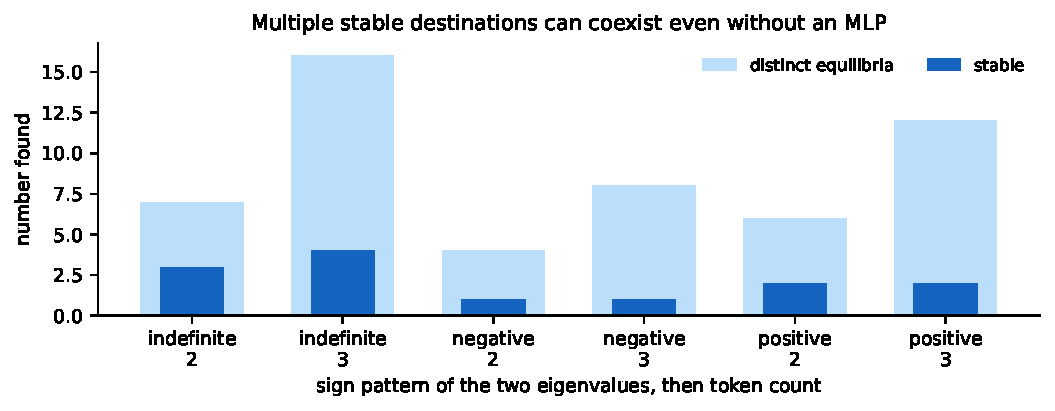
\includegraphics[width=0.9\textwidth]{../non_mlp_cycles_paper/figures_en/small_equilibrium_catalogue.pdf}
\caption{Numerically recovered stationary configurations for three spectra in the
tied symmetric planar model.  The plotted catalogue is not claimed complete.
\Cref{thm:spectral-gram} gives the complete implicit stationary system; solving every
branch of that transcendental system is a separate problem.}
\label{fig:equilibrium-catalogue}
\end{figure}

\section{Fixed points, periodic orbits, and the continuous-depth limit}
\label{sec:exact-equations}

\subsection{Finite-layer fixed points}

\begin{proposition}[Necessary and sufficient condition for a finite layer]
A configuration $X$ is a fixed point of \eqref{eq:serial-layer} if and only if, for
every token, there exist a unit intermediate point $y_i$ and two strictly positive
numbers $r_i,s_i$ such that
\begin{equation}
 x_i+hA_i(X)=r_i y_i,\qquad
 y_i+hM(y_i)=s_i x_i.\label{eq:finite-fixed}
\end{equation}
\end{proposition}

\begin{proof}
The first equality states exactly that the first normalization produces $y_i$; the
second states that the second normalization returns to $x_i$. Positivity of $r_i$ and
$s_i$ preserves rather than reverses direction. Conversely, normalizing both
equalities recovers \eqref{eq:serial-layer} and then $F_i(X)=x_i$.
\end{proof}

This form retains the softmax exponential inside $A_i$ but removes the normalization
divisions. It can therefore be used directly by an equation solver.

\subsection{Finite-layer periodic orbits}

For period $p$, introduce $X^k,Y^k\in(\sphere^{d-1})^n$ and
$r_i^k,s_i^k>0$ for $k=0,\ldots,p-1$. Write \eqref{eq:finite-fixed} at every step, replace the final
$X$ by the next state, and close the loop:
\begin{align}
 x_i^k+hA_i(X^k)&=r_i^k y_i^k,\\
 y_i^k+hM(y_i^k)&=s_i^k x_i^{k+1},\\
 X^p&=X^0.\label{eq:all-cycles}
\end{align}
To require primitive period, exclude returns before $p$. These equations therefore
cover arbitrary periods and configurations, including nonpolygonal orbits.

\subsection{Continuous-depth equation}

For a unit vector $x$ and a push $z$,
\[
 \N(x+hz)=x+h(I-xx^{\T})z+O(h^2).
\]
Applying this identity twice to \eqref{eq:serial-layer} gives
\begin{equation}
 \boxed{\quad\dot x_i=(I-x_ix_i^{\T})\{A_i(X)+M(x_i)\}.\quad}\label{eq:continuous}
\end{equation}
Liu and Herty identify this serial attention--MLP architecture as a Lie--Trotter
splitting of the summed continuous equation \cite{herty2026meanfield}.  The local
calculation below records the order at which the two possible layer orderings first
differ.
Serial ordering appears only in the order-$h^2$ term. All continuous equilibria are
therefore exactly the solutions of
\begin{equation}
 \boxed{\quad(I-x_ix_i^{\T})\{A_i(X)+M(x_i)\}=0,
 \qquad i=1,\ldots,n.\quad}\label{eq:continuous-equilibrium}
\end{equation}

More explicitly, let the normalized attention and MLP submaps have local expansions
\[
 R_{A,h}=I+hf+h^2r_A+O(h^3),\qquad
 R_{M,h}=I+hg+h^2r_M+O(h^3),
\]
where $f_i=P_{x_i}^{\perp}A_i$ and $g_i=P_{x_i}^{\perp}M(x_i)$.  Then
\begin{align}
 R_{M,h}\circ R_{A,h}
 &=I+h(f+g)+h^2\{r_A+r_M+Dg[f]\}+O(h^3),\\
 R_{A,h}\circ R_{M,h}
 &=I+h(f+g)+h^2\{r_A+r_M+Df[g]\}+O(h^3).
\end{align}
Their difference is
$h^2(Dg[f]-Df[g])+O(h^3)$.  The serial block and a parallel continuous control share
the first-order vector field, while finite layers retain this commutator correction.

At equilibrium the total push may be nonzero, provided that it is parallel to the
token. Attention and the MLP may cancel in tangent directions even when neither
subfield vanishes separately.

\subsection{Stability}

The stability calculation perturbs every token along tangent directions to its
sphere.  For a finite layer, spectral radius strictly below one for the restricted
derivative implies local asymptotic stability, whereas an eigenvalue of modulus
greater than one implies instability.  For the continuous flow, negative spectral
abscissa of the tangent Jacobian implies local asymptotic stability, whereas a
positive real part implies instability.  Eigenvalues on the unit circle or imaginary
axis require higher-order analysis.  The full tangent calculation includes
perturbations that separate temporarily equal tokens.

\section{Finite-layer census}
\label{sec:taxonomy}

The four families combine two choices for attention with two choices for the MLP.
\begin{center}
\begin{tabularx}{0.9\textwidth}{cYY}
\toprule
Type & Attention & MLP \\
\midrule
1 & $S=V=V^{\T}$ & potential \\
2 & $S=V=V^{\T}$ & general quadratic \\
3 & untied $S$ and $V$ & potential \\
4 & untied $S$ and $V$ & general quadratic \\
\bottomrule
\end{tabularx}
\end{center}

For types 3 and 4, we separated four subcases: symmetric $S$ and $V$; symmetric $S$
and general $V$; general $S$ and symmetric $V$; and both general. MLP widths are
1, 2, 4, and 8; the main inventory uses one to four tokens.

The first broad sweep contains 28,672 models, with 96 starts per model and hence
2,752,512 trajectories.  Families 1, 2, and 4 use 1,024 models at each token count;
family 3 uses 4,096.  Step size, sharpness, and the ratio of attention to MLP scale
are continuous random variables.  The five reported ranges for each quantity are
post-hoc bins, not a factorial parameter grid.  The ensemble and decision rules are
specified in \cref{sec:numerical-ensembles}.  The sweep is a finite sample from that
law, not an enumeration of the continuous matrix space.

\subsection{Stable fixed points}

Direct equation solving finds the following mean numbers of stable fixed points.
\begin{center}
\begin{tabular}{c@{\quad}ccc@{\qquad}c}
\toprule
Type & 1 token & 2 tokens & 3 tokens & observed maximum \\
\midrule
1 & 1.68 & 2.34 & 3.09 & 8 \\
2 & 1.49 & 2.03 & 2.55 & 9 \\
3 & 1.57 & 2.13 & 2.61 & 8 \\
4 & 1.31 & 1.71 & 2.00 & 7 \\
\bottomrule
\end{tabular}
\end{center}

In the decoupled planar model with
$\phi(\theta)=(g/3)\cos(3\theta)$ and $g>0$, each token obeys
$\dot\theta=-g\sin(3\theta)$.  It has exactly three stable wells, hence exactly $3^n$
stable labeled product equilibria.  All $3^n$ hyperbolic branches persist for
sufficiently weak coupling by the implicit-function theorem.  At coupling $0.03$,
seeded solves numerically continue 3, 9, 27, 81, and 243 distinct stable fixed points
for one through five tokens.  These counts are lower bounds at that finite coupling
because the solves do not exclude additional roots.

\subsection{Three- and four-layer cycles}

The broad trajectory screen assigned period-three and period-four labels by numerical
recurrence tests.  Its raw counts are:
\begin{center}
\begin{tabular}{crrrr}
\toprule
Type & screened p3 trajectories & p3 models & screened p4 trajectories & p4 models \\
\midrule
1 & 321 & 8 & 201 & 15 \\
2 & 2,039 & 34 & 1,823 & 28 \\
3 & 4,490 & 75 & 4,507 & 113 \\
4 & 1,621 & 22 & 1,860 & 41 \\
\bottomrule
\end{tabular}
\end{center}

These counts are screening labels, not 8,862 equation-level certificates.  For each
of the eight type--period pairs, one stored representative was subsequently refined by
solving $F^p(X)=X$.  All eight representatives have residual below
$5\times10^{-15}$, no earlier return, and spectral radius below one for the derivative
of $F^p$.  The screen estimates how often its recurrence classifier fired under the
sampled ensemble; the refinement establishes one stable primitive example in each
cell.

The extended atlas contains numerically resolved primitive candidates at every period
from 5 through 12.  These occur across all four tested MLP widths and also under
uniform attention ($\beta=0$), but they are not all stable; in particular, the stored
type-1 period-12 orbit is unstable.  A general MLP alone can produce stable p3 and p4
cycles. A potential MLP alone produced no verified p3 in 65,536 trajectories, and its
only p4 candidate reduced to a shorter period.

\begin{figure}[t]
\centering
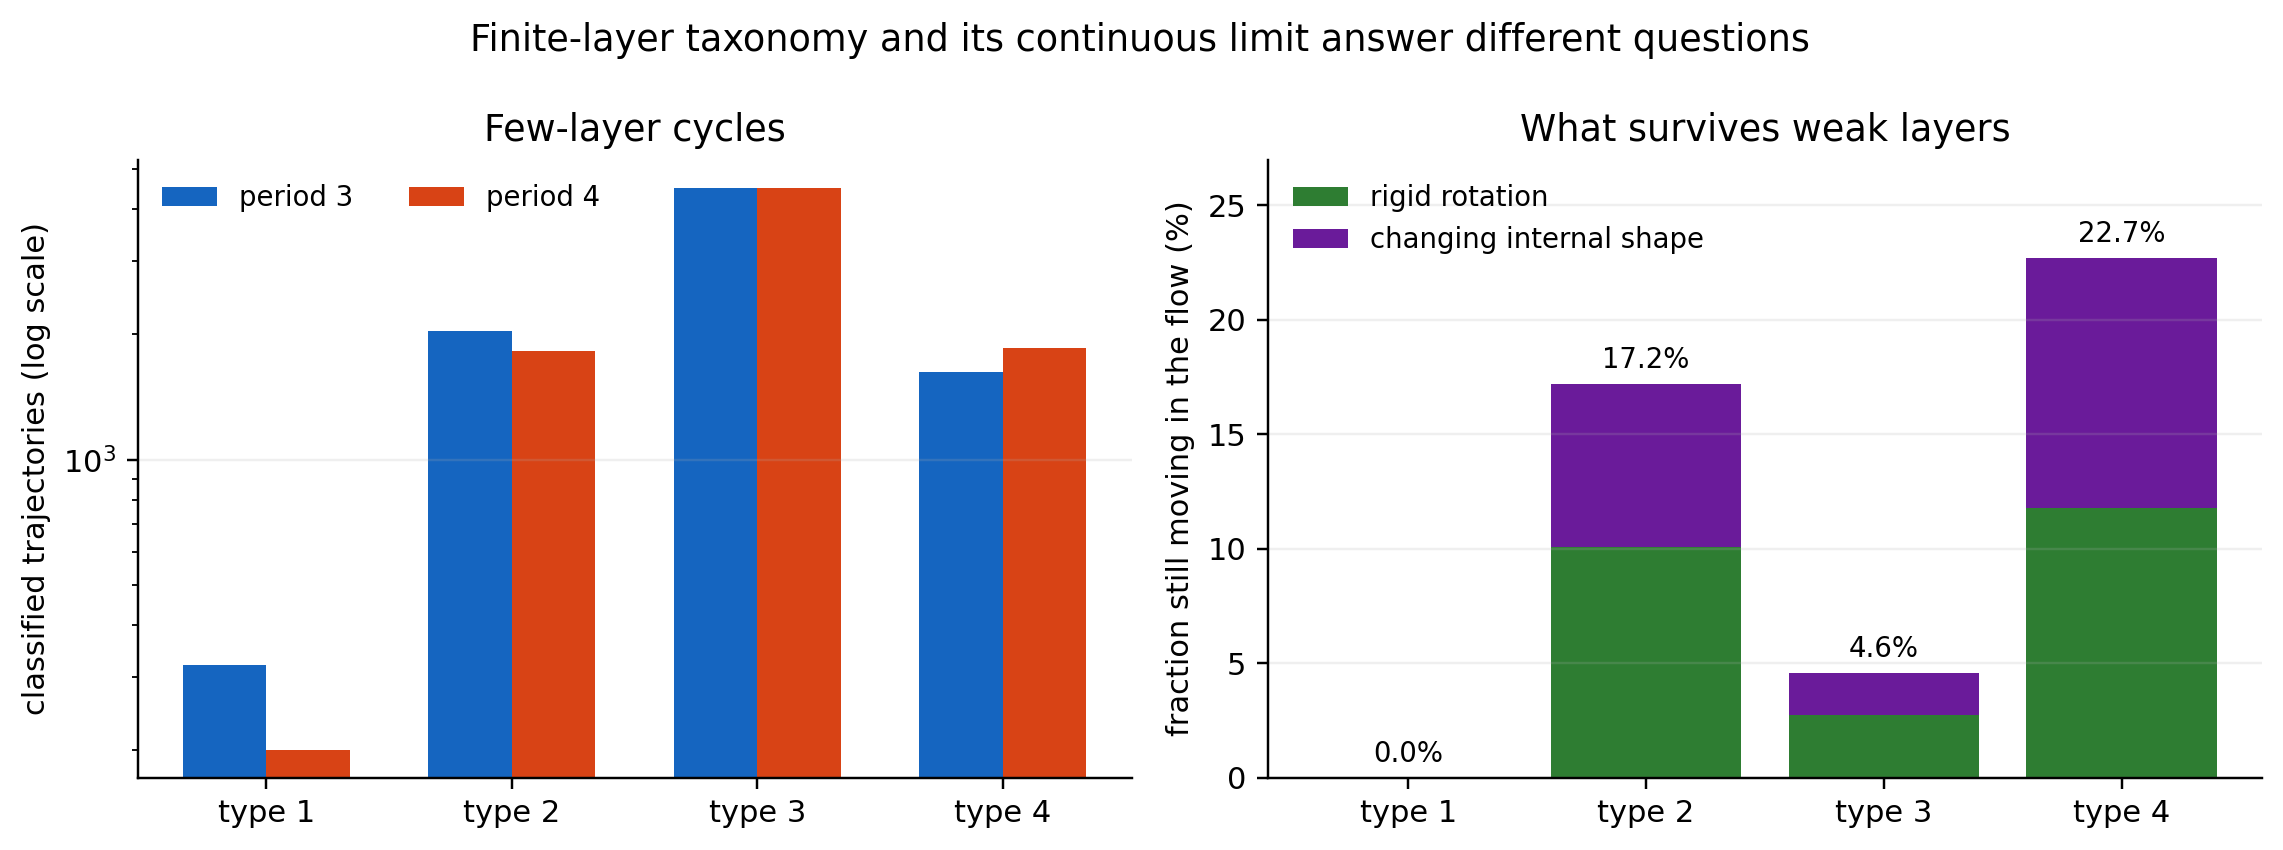
\includegraphics[width=\textwidth]{figures_en/taxonomy_and_survival.png}
\caption{Left: few-layer cycles in the first sweep. Right: fraction of selected
attractors that remains mobile after passing to the continuous equation. The panels
have neither the same denominator nor the same question.}
\label{fig:taxonomy-survival}
\end{figure}

At finite step size, composing two normalized substeps can create a periodic orbit
even when their infinitesimal vector fields are separately gradient-like.  The
finite-step normalization need not preserve either infinitesimal energy.  In the
continuous-depth limit, recurrence depends on circulation in the sum of the two
vector fields.

\section{Weak-layer limit}
\label{sec:small-step}

Suppose $F_h=I+hf+O(h^2)$. For a fixed integer period $p$,
\begin{equation}
 F_h^p(x)=x+phf(x)+O(h^2).\label{eq:fixed-period-collapse}
\end{equation}
A cycle that remains exactly three or four layers long as $h$ tends to zero can only
accumulate near a point where $f(x)=0$. A genuine continuous cycle can survive, but
the number of layers required for one revolution must grow as $T/h$, where $T$ is its
physical return time.

Fix the parameters, an initial condition, and $T<\infty$.  Suppose that the two
normalization inputs remain nonzero on a compact neighborhood of the corresponding
flow segment, so that the local defect and its first derivative are uniformly
bounded.  Then, for sufficiently small $h$, the serial layer satisfies
\begin{equation}
 \max_{0\le k\le \lfloor T/h\rfloor}\norm{F_h^k(X)-\varphi_{kh}(X)}=O(h),\label{eq:finite-time}
\end{equation}
where $\varphi_t$ is the flow of \eqref{eq:continuous}. This convergence does not
guarantee that two chaotic trajectories remain close forever. It guarantees that the
continuous equation is the correct limit on every fixed time window. Trajectory
distributions and basins are therefore checked separately.

\subsection{Numerical protocol}

The complete audit contains:
\begin{itemize}
  \item 214,528 model configurations and 2,844,160 initial trajectories;
  \item 26,112 fresh, unselected controls in the 24 cells obtained by crossing the
  four types with 1, 2, 3, 4, 8, and 16 tokens;
  \item 23,789,394,642 model--layer updates, or 102,108,101,290 token--layer updates;
  \item 307,200,000 reference RK4 evaluations, or 1,740,800,000 token--field evaluations;
  \item steps down to $h/4096$, two nondyadic grids, physical times 2, 10, and 20, and
  Richardson controls that cancel the first-order error.
\end{itemize}

The error slope is $1$ in every family. After Richardson cancellation it is $2.018$
over the main population. At the finest step, the median error falls from
$2.63\times10^{-4}$ to $3.39\times10^{-7}$. These measurements support the
first-order expansion $F_h=I+hf+h^2g+\cdots$ on the sampled parameter sets.

\subsection{Continuous-flow classification}

The 1,908 selected attractors are replayed directly under \eqref{eq:continuous}.
\begin{center}
\begin{tabular}{crrrrr}
\toprule
Type & replayed & fixed & moving & rigid rotation & changing internal shape \\
\midrule
1 & 286 & 286 & 0 & 0 & 0 \\
2 & 378 & 313 & 65 & 38 & 27 \\
3 & 768 & 732 & 36 & 21 & 15 \\
4 & 476 & 368 & 108 & 55 & 53 \\
\midrule
Total & 1,908 & 1,699 & 209 & 114 & 95 \\
\bottomrule
\end{tabular}
\end{center}

Thus 89.0\% of the complex finite-step attractors selected become fixed points, while
11.0\% remain mobile over the main window. This rate is conditional on selecting a
complex attractor; it is not their frequency among all random matrices.  The table
uses the strengthened replay with two perturb-and-relax stages.  One numerical
synchronization lock was reclassified as moving after a longer recheck, and one
moving type-4 record was reclassified from rigid to internal motion.  Before these
audited corrections the same window gave 1,700 fixed, 208 moving, and 93 internal
records.

For 8 and 16 tokens, 581 candidates are continued. At step $h/4096$, the raw count is
118 moving states. Four apparently fixed states have an unstable direction hidden by
numerically identical tokens; after correction, the finite map and continuous flow
both give 122 moving states and agree case by case in 575 of 581 instances. The six
remaining differences select coexisting basins.

\section{Recurrent dynamics in the continuous flow}
\label{sec:attractors}

\subsection{An exact type-3 limit cycle}

Let $d=2$, write $x(\theta)=(\cos\theta,\sin\theta)$, and let $J$ denote rotation by
$\pi/2$.  Take uniform attention, $S=0$, value transport
$V=aI+\omega J$ with $a>0$, and the potential MLP
\begin{equation}
 \phi(x)=\frac{g}{3}\operatorname{Re}(x_1+\mathrm i x_2)^3.
 \label{eq:triwell-potential}
\end{equation}

\begin{proposition}[Orbitally stable active rotator]
\label{prop:active-rotator}
If $|\omega|>|g|$, the synchronized manifold
$x_1=\cdots=x_n=x(\theta)$ is an exact periodic orbit of
\eqref{eq:continuous}.  Its phase satisfies
\begin{equation}
 \dot\theta=\omega-g\sin(3\theta),\qquad
 T=\frac{2\pi}{\sqrt{\omega^2-g^2}}.
 \label{eq:active-rotator}
\end{equation}
The collective Floquet exponent is zero and all $n-1$ transverse exponents equal
$-a$.  The orbit is therefore locally orbitally asymptotically stable.
\end{proposition}

\begin{proof}
At synchrony the uniform attention output is
$a x(\theta)+\omega Jx(\theta)$.  Its radial part disappears under projection, while
the tangential part of $\nabla\phi$ is $-g\sin(3\theta)$, which gives
\eqref{eq:active-rotator}.  The standard integral over one rotation gives the stated
period.  Write $\theta_i=\theta+\eta_i$.  To first order,
\[
 \dot\eta_i=a(\bar\eta-\eta_i)-3g\cos(3\theta)\eta_i.
\]
The collective component is the phase variation.  For every zero-mean transverse
component the instantaneous rate is $-a-3g\cos(3\theta)$.  The second term has zero
period average because
\[
 \int_0^{2\pi}\frac{\cos(3\theta)}
 {\omega-g\sin(3\theta)}\,d\theta=0.
\]
Hence every transverse Floquet exponent is $-a$.
\end{proof}

For the experimental values $a=1.2$, $\omega=0.8$, and $g=0.25$, the exact mean
angular speed is $\sqrt{\omega^2-g^2}=0.759934\ldots$.  The 128-start simulations
measure the basin reached by the serial discretization; they are not needed for the
existence or local stability of the continuous orbit.

\subsection{Stable cycles}

Four recurrent motions are numerically resolved in the block with an MLP: one p3 and
one p4 seed from type 2, followed by one p3 and one p4 seed from type 4.  At the
deepest dyadic steps, their full labeled-state return times agree with RK4:
respectively $16.632$ versus $16.660$, $9.331$ versus $9.340$, $9.389$ versus
$9.400$, and $6.4395$ versus $6.4400$.  On nondyadic grids, fitted layer-count
exponents are $1.0016$, $1.0029$, $0.9992$, and $0.9950$.  The second fit uses a
Gram/shape return; it does not by itself validate a full-state period.  Perturbed
trajectories return to the same recurrent motion in every robustness run.

The type-4 p3 case is especially informative: attention alone retains the cycle while
the MLP alone stops.  With the MLP removed, its stored parameters are
\begin{equation}
 \begin{aligned}
 S&=\begin{pmatrix}1.112495&1.768642\\-2.540753&3.294286\end{pmatrix},\\
 V_0&=\begin{pmatrix}-1.809502&1.419182\\-1.827949&-3.611608\end{pmatrix},\\
 \beta&=1.110063,& \rho&=0.551488.
 \end{aligned}
 \label{eq:attention-cycle-matrices}
\end{equation}
The audit uses normalized depth $\tau$ and integrates
$dX/d\tau=\rho f_{S,V_0,\beta}(X)$.  This is the flow
\eqref{eq:attention-flow} after the time change $t=\rho\tau$, or equivalently after
replacing $V_0$ by $\rho V_0$.  Independent RK4 integration gives return time
$T_\tau=9.120$ and hence $T_t=5.02957$ in the convention of
\eqref{eq:attention-flow}.  The pairwise inner products range from $-0.8002$ to
$-0.0551$, excluding a rigid rotation.  Over 2,000 units of $\tau$, the Benettin--QR
estimate of the Lyapunov spectrum per unit $\tau$ is
\begin{equation}
 (-0.00273,-0.45676,-0.45937),
 \label{eq:attention-cycle-spectrum}
\end{equation}
or $(-0.00495,-0.82823,-0.83296)$ per unit $t$.  The first rate approximates the
neutral phase direction.  For 128 Gaussian angular perturbations of standard
deviation $0.08$, the maximum phase-minimized distance after 36 units of $\tau$ is
$0.003673$ radians, compared with a maximum initial distance of $0.142421$.  Across
seven dyadic and nondyadic layer ratios, the fitted slope of layers per revolution
against inverse layer strength is $1.012$.  These tests are consistent with convergence to an attracting
continuous-depth periodic orbit; they are not a computer-assisted existence proof.

\begin{figure}[t]
\centering
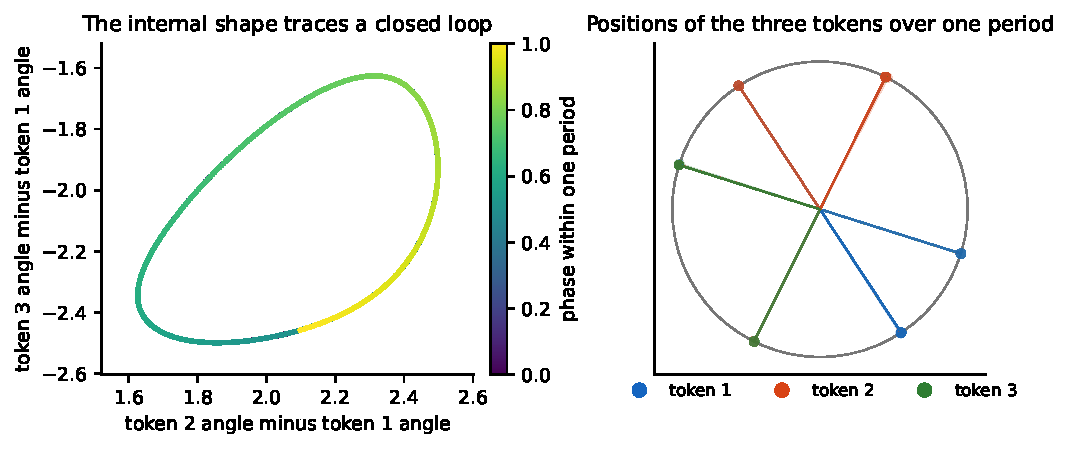
\includegraphics[width=0.92\textwidth]{../non_mlp_cycles_paper/figures_en/attention_only_cycle_geometry.pdf}
\caption{Numerically resolved attracting internal cycle under attention alone.  The
relative-angle curve is nonconstant, and seven phases show the changing three-token
geometry.}
\label{fig:attention-only-cycle}
\end{figure}

In the other three numerically resolved recurrent examples, the MLP participates in
the motion.

\subsection{Three-token chaotic-attractor candidates}

Here a motion is called chaotic only after four checks: one perturbation direction
grows on average; one direction remains neutral because it follows time along the
trajectory; the remaining directions contract; and the sum of rates agrees with the
independently computed mean divergence.

The three-token type-4 case has rates
\[
 (0.1489,\ 0.0007,\ -0.3923).
\]
The leading rate remains positive in all 24 perturbations and for three RK4 steps; at
step $0.005$ it equals $0.1584$. All 512 tested uniform starts reach an internal motion
with positive rate within the stated observation window. Attention alone stops, the
MLP alone produces a regular rotation, and their interaction gives strong numerical
evidence of chaos.

A second type-2 example has rates
\[
 (0.0333,\ -0.0011,\ -0.7253).
\]
Here attention alone and the MLP alone both stop. Among 512 starts, 449 exceed the
strict $0.03$ threshold and the other 63 remain positive between $0.022$ and $0.03$.

\subsection{An eight-token hyperchaotic-attractor candidate}

One type-4 example has three independent separating directions:
\[
 (0.1458,0.1455,0.1435,0.0031,-0.0409,
 -0.1871,-0.1872,-0.1896).
\]
A replication with a step twice as small retains three positive rates. Four tokens
remain synchronized during this motion; the trajectory alternates mainly between
$4+4$ and $4+3+1$ partitions. It is a chimera: one part of the group remains ordered
while group phases evolve unpredictably. Attention weights vary very little, whereas
token geometry varies strongly.

\begin{figure}[t]
\centering
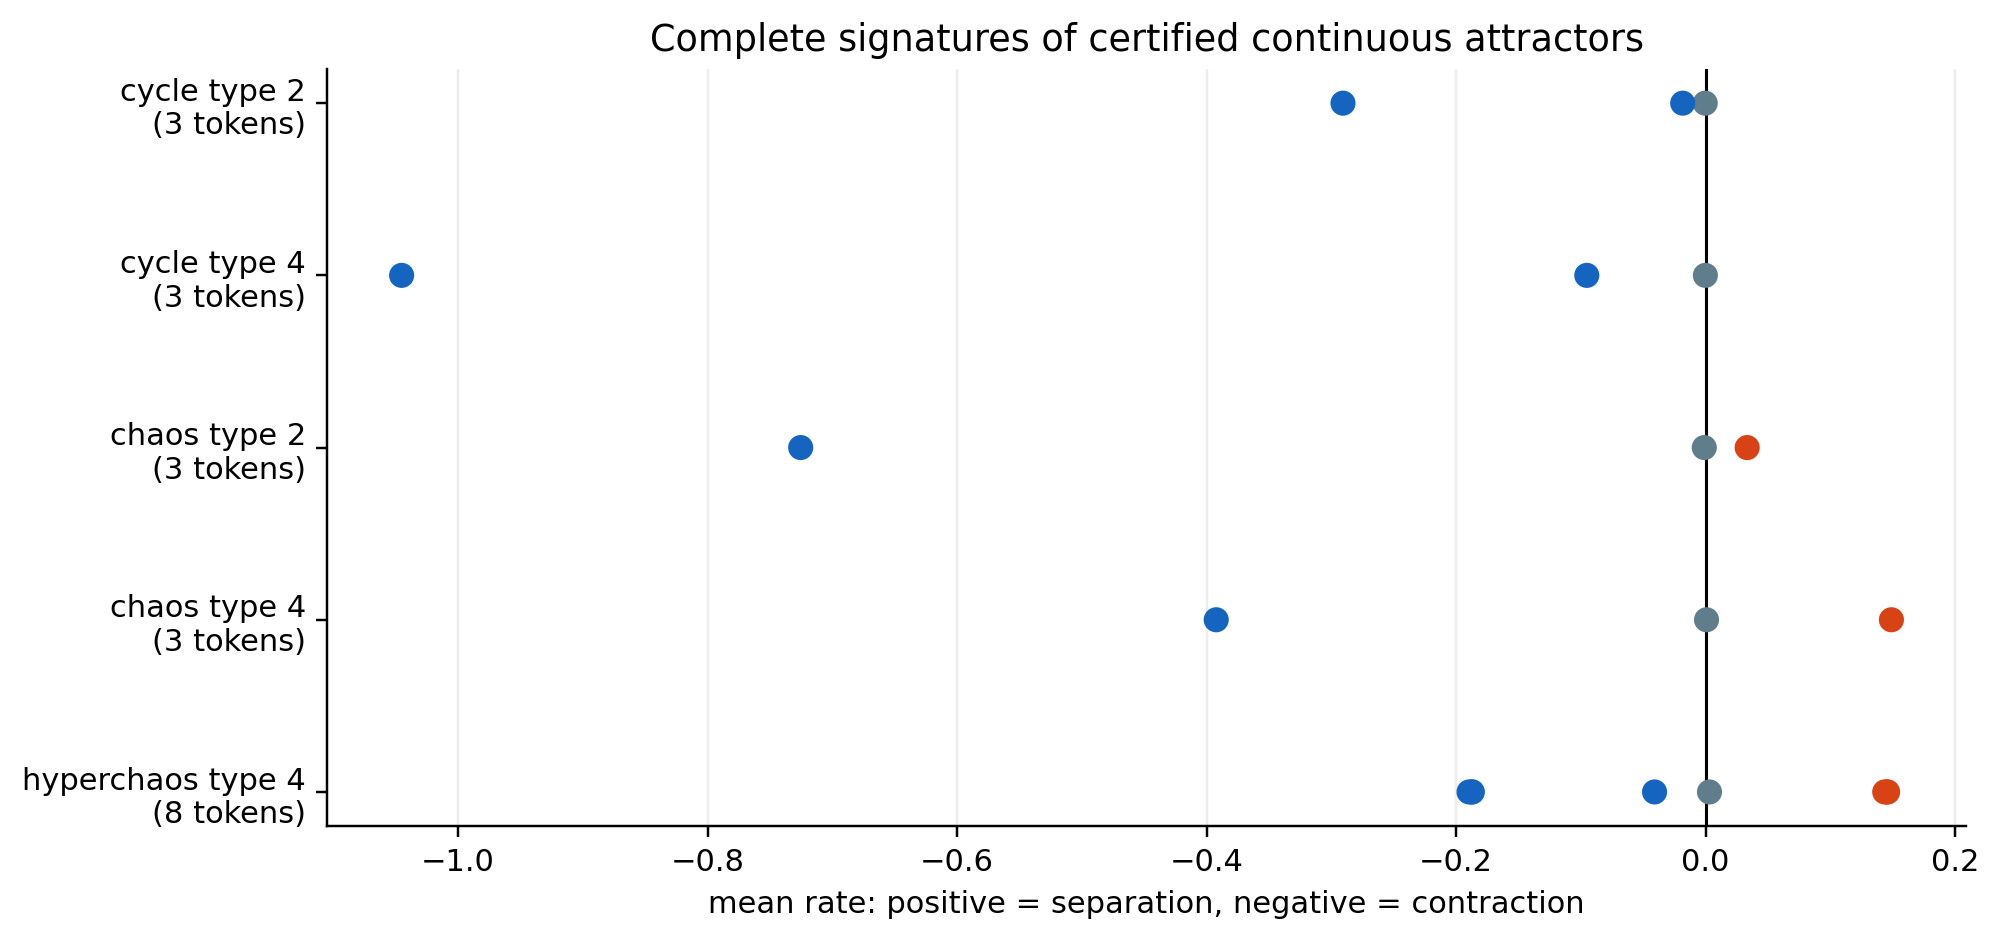
\includegraphics[width=0.92\textwidth]{figures_en/continuous_spectra.png}
\caption{Complete rates for cycles and chaotic-attractor candidates. An orange point to the
right of zero means that a small difference grows; a blue point to the left means it
contracts; a gray point near zero follows the phase of the motion.}
\label{fig:spectra}
\end{figure}

Tomihari and Karakida previously used state Jacobians and finite-time Lyapunov
exponents for normalized recurrent self-attention, including nonsymmetric and
multihead layers \cite{tomihari2025recurrent}.  They show that normalization can keep
the Jacobian spectrum near criticality and report slightly positive maximum
finite-time exponents, with larger values in some multihead models.  Their horizon is
$T=16$ and their quantity does not establish an asymptotic chaotic attractor.  Our
long-horizon spectra, divergence checks, and perturbation ensembles address that
numerical distinction, while still falling short of a computer-assisted proof.  The
exact active rotator above supplies an existence theorem for a periodic orbit, not for
the chaotic examples.

\subsection{Recurrent motion under uniform attention}

At $\beta=0$, every weight always equals $1/n$. Nevertheless, a four-token type-3
case retains intermittent motion with positive leading rate. The source is
the antisymmetric part of $V$. Replacing it by its symmetric part, removing attention,
or removing the MLP causes convergence to a fixed point. In an audit of 512 starts,
the same weight set has fixed points, recurrent motions, and positive-rate trajectories:
initialization selects the basin.

On the circle, this case rewrites exactly as a system of coupled oscillators. The
antisymmetric part of $V$ supplies the tendency to rotate, while the potential MLP
supplies regions where motion slows. Uniform attention is therefore not an absence of
interaction; it is coupling through the global mean.

No robust quasiperiodic torus was found in the audited sample. The observed classes include fixed points,
stable spirals, periodic orbits, and trajectories with numerical signatures of chaos
or hyperchaos.  This is not an exhaustive classification of a high-dimensional
continuous system.

\section{Potential structure and circulation}
\label{sec:energy}

When $\beta=0$, $V=V^{\T}$, and the MLP is potential, the function
\begin{equation}
 \Phi(X)=\frac{1}{2n}\sum_{i,j}x_i^{\T}Vx_j+\sum_i\phi(x_i)\label{eq:global-potential}
\end{equation}
increases along trajectories:
\[
 \frac{d\Phi}{dt}=\sum_i\norm{(I-x_ix_i^{\T})\nabla_{x_i}\Phi}^2\ge0.
\]
A nonconstant loop would return to the same value after a revolution despite having
strictly increased, which is impossible. All 146 numerical trajectories in this
exact-potential control were classified as converged on the stated observation
window.

Row-wise softmax normalization can break this simple structure even when
$S=V=V^{\T}$. Among 1,699 audited equilibria, 28 are stable spirals: one in type 1,
19 in type 3, and eight in type 4; none appears in the exact $\beta=0$ control. The
single type-1 spiral shows that two symmetric subfields with different mobilities do
not guarantee a single Euclidean energy.

For unnormalized multihead attention, properly aligned symmetric heads add into a
common energy. With separate normalizations, this conclusion needs additional
conditions because each head multiplies its push by its own denominator. Massucco and
collaborators give an energy with a nonlocal mobility for a specified tied
time-dependent setting \cite{massucco2026time}.  Rodr\'iguez Abella, Silvestre, and
Tabuada prove consensus for bounded, uniformly continuous time-dependent score
matrices and any
number of independently normalized heads when every transported output is the
identity and the tokens begin in a common hemisphere
\cite{rodriguez2025asymptotic}.  Our examples leave those hypotheses through general
output matrices, untied transport, or token configurations spanning more than one
hemisphere.

\section{Multihead equilibria and basin geometry}
\label{sec:multihead}

For $L$ heads, the push is
\begin{equation}
 A_i^{\mathrm{multi}}(X)=\sum_{\ell=1}^{L}\omega_\ell
 \sum_j a_{ij}^{(\ell)}(X)C_\ell x_j.\label{eq:multihead}
\end{equation}
The score matrix of head $\ell$ determines its weights; $C_\ell$ includes its value matrix
and output recombination. The destination satisfies
\[
 (I-x_ix_i^{\T})\{A_i^{\mathrm{multi}}(X)+M(x_i)\}=0.
\]
Each head need not vanish separately. Two heads can cancel along the sphere and create
a destination that exists for neither head alone.

\subsection{Conditional basin maps}

We fix five tokens on the circle and allow a sixth probe to move. With two matrices
having the same spectrum $(2,-3)$ but axes rotated by 60 degrees, head A has four
destinations, head B has five, and their sum has seven. On the sphere the counts are
four, four, and five. The sum cuts boundaries, moves destinations, and creates small
basins. Two very close initial points can therefore end in distant groups if they lie
on opposite sides of a boundary.

\begin{figure}[t]
\centering
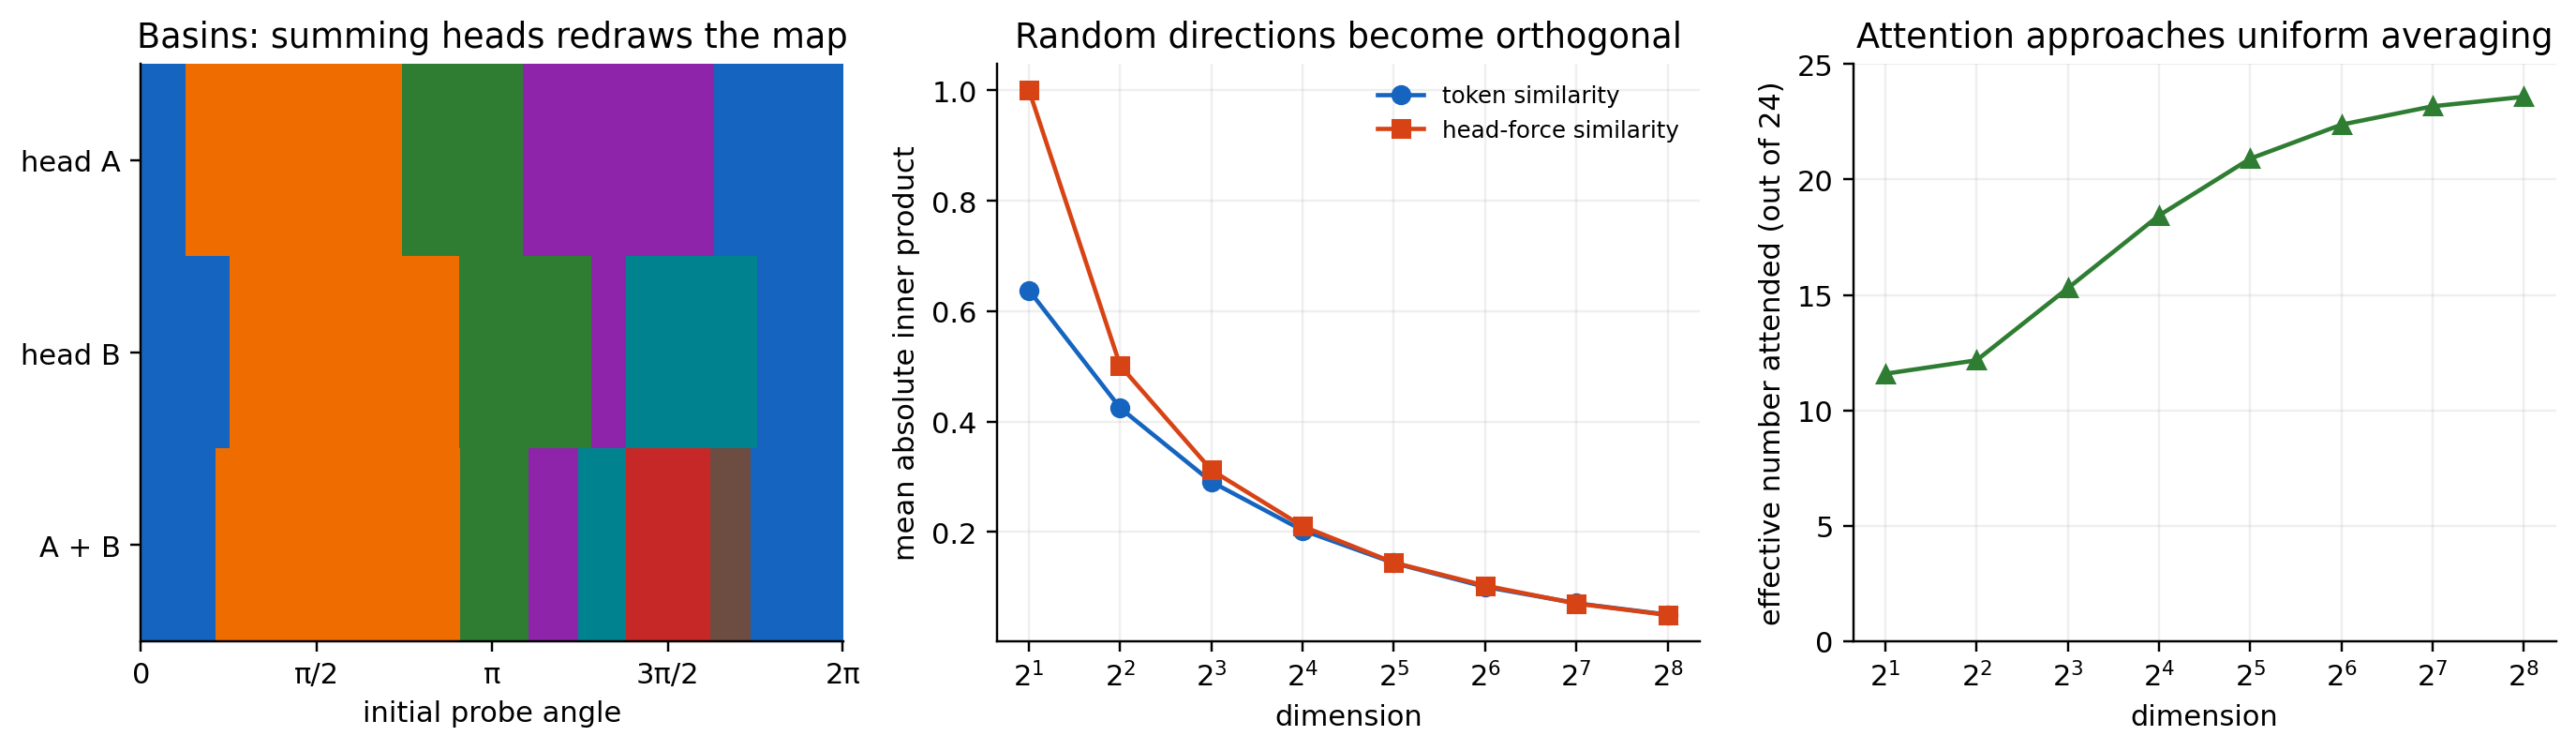
\includegraphics[width=\textwidth]{figures_en/multihead_and_dimension.png}
\caption{Left: probe destination as a function of its initial angle for head A, head B,
and their sum. Center: mean absolute inner products between tokens and between head
forces. Right: effective number of attended tokens, defined as the exponential of
the row-attention entropy. The experiment uses 24 tokens,
six random heads, and 96 repetitions per dimension.}
\label{fig:multihead-dimension}
\end{figure}

\subsection{Settling-time maps and fractal diagnostics}

Lai, Bao, Quinn, and Gilpin recently reported fractal settling-time maps, called
basin plots in their paper, for trained recurrent reasoning models
\cite{lai2026fractal}.  Their construction fixes a model and a task,
chooses a random two-dimensional plane in the full latent space, and colors each
initial condition by the number of recurrent loops until the decoded output stops
changing.  Consequently, adjacent colors may represent different transient durations
on routes to the same final answer.  Across their population plots, basin entropy
increases with the mean loop count on the same slice; examples ordered by
task-specific difficulty also follow this trend.  They attribute the long transients
to trajectories lingering near unstable, nearly correct states.  These correlations
do not constitute a complexity lower bound.  They repeat spatial
zooms and estimate uncertainty exponents.  For an Equilibrium Reasoner on Sudoku, the reported
values are $0.249$, $0.243$, and $0.216$ across the base, tenfold, and hundredfold
views; a Parcae example on Countdown and a Fixed-Point Reasoning Model example on
mazes give substantially larger values, roughly $0.85$--$0.91$.  Their finite latent
instability statistic compares neighboring decoded trajectories at finite separation.
In a separate toy training model they report finite-time Lyapunov exponents and
Jacobian eigendirections.

Their stopping rule is applied to the decoded answer.  A latent trajectory may still
move after its discrete decoding has stopped changing.  Our reduced model has no
task decoder, so the experiment below uses the norm of the token-state vector field
and records continuous settling time.  It is an analogue of their observable, not an
identical measurement.

Their training experiment supplies a second trend.  An eight-variable looped
Transformer for modular linear systems initially has several stable fixed points that
decode to incorrect solutions.  In four closely spaced reported checkpoints near
156,000 training steps, these states lose stability, the correct solution becomes the
common destination, basin entropy rises, and unstable Jacobian directions appear.
Positive finite-time exponents occur in variables requiring multistep elimination,
not in variables solved by direct substitution.  These measurements show a
coincident inference-space bifurcation and gain in task accuracy for that trained
model.  They do not establish that computational hardness forces the same transition
in every architecture.

Their population statistics use $200\times200$ slices, pixel separations one through
five, at least 300 valid slices per model--task pairing, and retain only slices for
which at least $90\%$ of starts reach the final solution and at most $1\%$ hit the
iteration cap.  The supplemental zooms produce stable or drifting fitted exponents,
which the authors interpret respectively as scale-stable and ``slim'' fractals.  A
repeated co-moving zoom is itself subject to the smooth-saddle null derived below.
This distinction is relevant for dissipative dynamics: convergence to one final
state does not force the settling-time field to have a smooth boundary
\cite{motter2013doubly,chen2017slim}.

The relation between constraint solving and transient chaos predates recurrent
reasoners.  Ercsey-Ravasz and Toroczkai construct a continuous-time SAT solver whose
solution clusters are attractors and whose basin boundaries become fractal beyond a
constraint-density threshold \cite{ercseyravasz2011optimization}.  Daza et al.
introduced basin entropy to quantify final-state uncertainty and gave a sufficient
entropy criterion for fractal basin boundaries \cite{daza2016basin}.  These results
justify the dynamical diagnostics; they do not turn an arbitrary recurrent system
with an intricate basin plot into a solver for a hard problem.  Such a conclusion for
our model would require an explicit map from problem instances to $S,V,M$, a decoding
map from attractors to solutions, and a cost analysis that includes precision and
transient time.  Daza et al.'s sufficient criterion applies to genuine terminal-basin
labels; it does not certify a map colored only by settling time.

Our plot in \cref{fig:multihead-dimension} measures a different object.  It varies one
probe angle over 1,440 points and colors the terminal attractor identity.  Heads A and
B and their sum have respectively $(4,5,7)$ destinations and $(4,5,7)$ label
transitions around the circle.  This establishes multistability and head-induced
partition refinement.  It contains no repeated zoom and gives no evidence of a
fractal boundary.

The small-step continuation audit also measures a different exponent.  For two
potential landscapes, the fraction of initial states whose token partition differs
between a finite layer and the continuous flow scales approximately as $h^{0.946}$
and $h^{0.958}$ over the main range.  Here $h$ is layer strength, not a perturbation
of the initial condition.  The values are consistent with an $O(h)$ displacement of
a smooth codimension-one separatrix and cannot be interpreted as uncertainty
exponents.

A simple saddle and a chaotic saddle make different predictions.  Near a hyperbolic
saddle with unstable rate $\lambda_u>0$, local linearization gives the settling-time
singularity
\begin{equation}
 T(x)\simeq \frac{1}{\lambda_u}
 \log\frac{C}{\operatorname{dist}(x,W^s)},
 \label{eq:saddle-settling}
\end{equation}
where $W^s$ is its stable manifold.  A smooth hyperbolic intersection of $W^s$ with
a fixed planar slice has uncertainty exponent one in the asymptotic small-separation
limit even though adjacent pixels can have very different settling times.  For the
standard terminal-basin uncertainty test, an exponent below one under the usual
scaling assumptions indicates a boundary of dimension greater than one; recurrent
folding by a chaotic saddle is one mechanism that produces it
\cite{grebogi1983fractal}.  Long transients and
a visually intricate finite grid are therefore insufficient on their own.

A related test for our dynamics records both terminal attractor and settling time on
a two-dimensional state slice.  Write $\vartheta=(\theta_1,\theta_2)$ for
the two slice coordinates.  Repeated spatial magnifications can then estimate, for a
stated time threshold $\delta>0$,
\begin{equation}
 f_\delta(\varepsilon)=
 \Pr\!\left(|T(\vartheta)-T(\vartheta')|\geq\delta
 \mid\norm{\vartheta-\vartheta'}_2=\varepsilon\right)
 \asymp\varepsilon^{\alpha_\delta}.
 \label{eq:uncertainty-exponent}
\end{equation}
A pair is uncertain here only when its continuous settling times differ by at least
$\delta$; this is a coarsened analogue of comparing unequal integer loop counts.
A fitted exponent below one under repeated co-moving zooms is not sufficient.  For
the smooth-saddle law \eqref{eq:saddle-settling}, let $d>0$ denote the normal distance
on one side and compare $d$ with $d+\varepsilon$.  Then
\begin{equation}
 |T(d+\varepsilon)-T(d)|\geq\delta
 \quad\Longleftrightarrow\quad
 d\leq \frac{\varepsilon}{e^{\lambda_u\delta}-1}.
 \label{eq:smooth-saddle-null}
\end{equation}
The uncertain fraction is asymptotically proportional to $\varepsilon$ on a fixed
window, but it saturates when the right-hand side is comparable to the window width.
Shrinking the window and the pixel spacing by the same zoom factor preserves this
dimensionless ratio and can preserve a low finite-scale fitted slope for a perfectly
smooth stable manifold.  Evidence for a fractal boundary therefore requires
fixed-window resolution refinement beyond this saturation regime, in addition to
integration-step and horizon controls.  A positive finite-time tangent rate during
one saddle passage is also compatible with a smooth boundary; recurrent folding or
an invariant chaotic saddle requires separate evidence.  Terminal-attractor labels
require a separate basin-uncertainty calculation.  The tied symmetric continuous attention flow cannot contain a
nonstationary chaotic invariant set because of \eqref{eq:tied-energy-identity}; a
geometrically complicated field of slow settling near stationary saddles remains
possible.  Untied heads, a general MLP, or a finite recurrent map also admit recurrent
saddles.  The four-token untied example with 147 fixed and 365 moving or unresolved
outcomes among 512 starts is a candidate for this test; its existing sample does not
establish fractality.

A separate three-token type-2 candidate used for the atlas below also permits an
exact one-dimensional reduction.  On the synchronized manifold, write
$x(\theta)=(\cos\theta,\sin\theta)$ and
$x(\theta)^\perp=(-\sin\theta,\cos\theta)$, and let
$\rho=1.4468864491008047$ be the source record's overall depth scale.  Its angular
field is
\begin{equation}
 \dot\theta=g(\theta,\gamma)
 =\rho x(\theta)^{\perp\T}\{Vx(\theta)+\gamma M(x(\theta))\}.
 \label{eq:fractal-consensus-field}
\end{equation}
A numerical evaluation using 60-digit arithmetic on the stored decimal coefficients gives a
saddle--node at
\begin{align*}
 (\theta_c,\gamma_c)
 &= (1.1095854010814425,\,1.4347884764108496),\\
 g_\gamma&=0.2655849737,&
 g_{\theta\theta}&=-9.5222584300.
\end{align*}
This evaluation is neither symbolic nor interval-certified.  With
$u=\theta-\theta_c$ and $\mu=\gamma-\gamma_c$, Taylor expansion gives
\begin{equation}
 g(\theta_c+u,\gamma_c+\mu)
 =0.2655849737\mu-4.7611292150u^2
 +O(|u|^3+|\mu u|+\mu^2).
 \label{eq:fractal-saddle-node-normal-form}
\end{equation}
At the same numerical point, central differences of the full three-angle field give
the spectrum
\[
 (0,-0.05706479,-0.05706479).
\]
The zero collective direction and the two strictly contracting transverse directions
are consistent with a generic saddle--node of the full field.  This remains a
floating-point calculation rather than a computer-assisted proof.
For $\mu>0$, the predicted separation of the two synchronized roots is
$0.4723639672\sqrt\mu+O(\mu)$, and the magnitudes of their collective eigenvalues are
$2.2489858845\sqrt\mu+O(\mu)$.  At $\gamma=1.4348$, the stable collective eigenvalue
is $-0.00763411$, corresponding to a linear relaxation time of $130.99$; its other
two angular eigenvalues are both $-0.06530978$.  The companion saddle has spectrum
$(0.00763495,-0.04881867,-0.04881867)$.  This slow
scale can create sharp finite-resolution changes in settling time without a fractal
boundary.

The fold itself supplies a stronger null for the settling-time statistic.  At
$\mu=0$, the leading normal equation on its repelling side is
\begin{equation}
 \dot u=-a u^2,\qquad
 T(u)\sim\frac{1}{a|u|},\qquad a=4.7611292150.
 \label{eq:fold-settling-null}
\end{equation}
Put $s=|u|>0$ on this side of the fold and compare $s$ with $s+\varepsilon$.  For the
leading normal form,
\begin{align*}
 |T(s+\varepsilon)-T(s)|\geq\delta
 &\quad\Longleftrightarrow\quad
 s(s+\varepsilon)\leq\frac{\varepsilon}{a\delta},\\
 0<s\leq s_*(\varepsilon)
 &:=\frac{\sqrt{\varepsilon^2+4\varepsilon/(a\delta)}-\varepsilon}{2}
 \sim\sqrt{\frac{\varepsilon}{a\delta}}.
\end{align*}
For a sampling density that is continuous and positive at the fold, the uncertain
fraction is therefore $f_\delta(\varepsilon)=\Theta(\varepsilon^{1/2})$.  The exponent
is one half although the singular set is smooth.  When
$\mu>0$, the hyperbolic regime is recovered only within a distance much smaller than
\[
 r=\sqrt{g_\gamma\mu/a}
\]
from either root.  For the atlas value $\gamma=1.4348$,
$r=8.0175\times10^{-4}$ and the root separation is
$2r=1.6035\times10^{-3}$.  The deepest-window initial-angle separations range from
$1.9175\times10^{-4}$ to $3.0680\times10^{-3}$.  The preceding flow distorts these
separations before the bottleneck, so their comparison with $r$ only locates a
possible crossover.

The numerical atlas contains 30,656 integrated initial conditions.  The four
$64\times64$ primary windows contain respectively 4,096, 4,096, 4,088, and 4,010
  trajectories satisfying the finite-horizon speed-and-tail criterion.  A post-hoc comparison
with the synchronized roots rejects 0, 1, 2, and 17 additional endpoints because
they are closer to the saddle than to the stable root.  The remaining endpoints are
  consistent with one stable consensus.  The three clusters obtained by applying a
  $10^{-3}$ tolerance directly to all finite-time endpoints record positions along the
  weak synchronized direction and are not evidence for three attractors.

For $\delta=2$, the root-audited finite-scale slopes across magnifications
$1,8,64,512$ are
\[
 1.025\pm0.077,\qquad 0.855\pm0.057,\qquad
 0.715\pm0.022,\qquad 0.663\pm0.070.
\]
The quoted uncertainties are ordinary least-squares standard errors from five
correlated pixel offsets, not independent-sample confidence intervals.  At the
deepest zoom the slope changes from $0.480$ for $\delta=1$ to $1.262$ for
$\delta=10$.  Across the speed-based controls, halving the integration step changes
any fitted slope by at most $0.0030$, whereas changing the grid from $64^2$ to
$32^2$ changes a slope by as much as $0.417$ and extending the deepest control from
time 220 to 300 changes it by as much as $0.115$.  The exponent has therefore not converged with respect to the
spatial, time-threshold, and horizon choices.

The geometry at the two finest windows is simpler than the fitted slopes suggest.
At magnification 512, all 103 pixels excluded by the combined speed-and-root-distance
audit form one contiguous strip:
every column has one interval and two boundary crossings.  Affine fits to its lower
and upper pixel edges have root-mean-square residuals $0.282$ and $0.288$ pixel, and
the minimum-time ridge has residual $0.284$ pixel.  No repeated folding is resolved.
The largest finite-time tangent exponent is $-0.00892$ along the longest retained
trajectory and $-0.09724$ along a typical one; at $\gamma=1.43475$, just below the
fold, the audited trajectory gives $-0.04955$.  These values persist under halving
the step and reducing the perturbation from $10^{-7}$ to $10^{-8}$.  Positive local
stretching intervals occur, but the full audited intervals are contracting.

The parameter scan agrees with the scalar bifurcation.  None of the 576 base-grid
trajectories satisfies the speed-and-tail criterion by time 220 at
$\gamma\in\{1.4346,1.4347,1.43475\}$, while all 576 satisfy the speed-and-tail criterion at
each tested $\gamma\geq1.4348$.  Since the atlas parameter exceeds $\gamma_c$ by only
$1.1524\times10^{-5}$, critical slowing is expected.  In the analytic hyperbolic
null, a $64^2$ co-moving grid gives a fitted slope $0.0046$ for $\delta=2$ and the
same value at every zoom; fixed-window refinement gives $0.996$ at resolution 2,048
and $1.003$ at 4,096.  The fold null instead approaches one half, giving $0.564$ and
$0.519$ at those resolutions.  Low finite-scale slopes and their persistence under
co-moving zooms therefore occur for smooth sets in both relevant local models.

\begin{figure}[t]
\centering
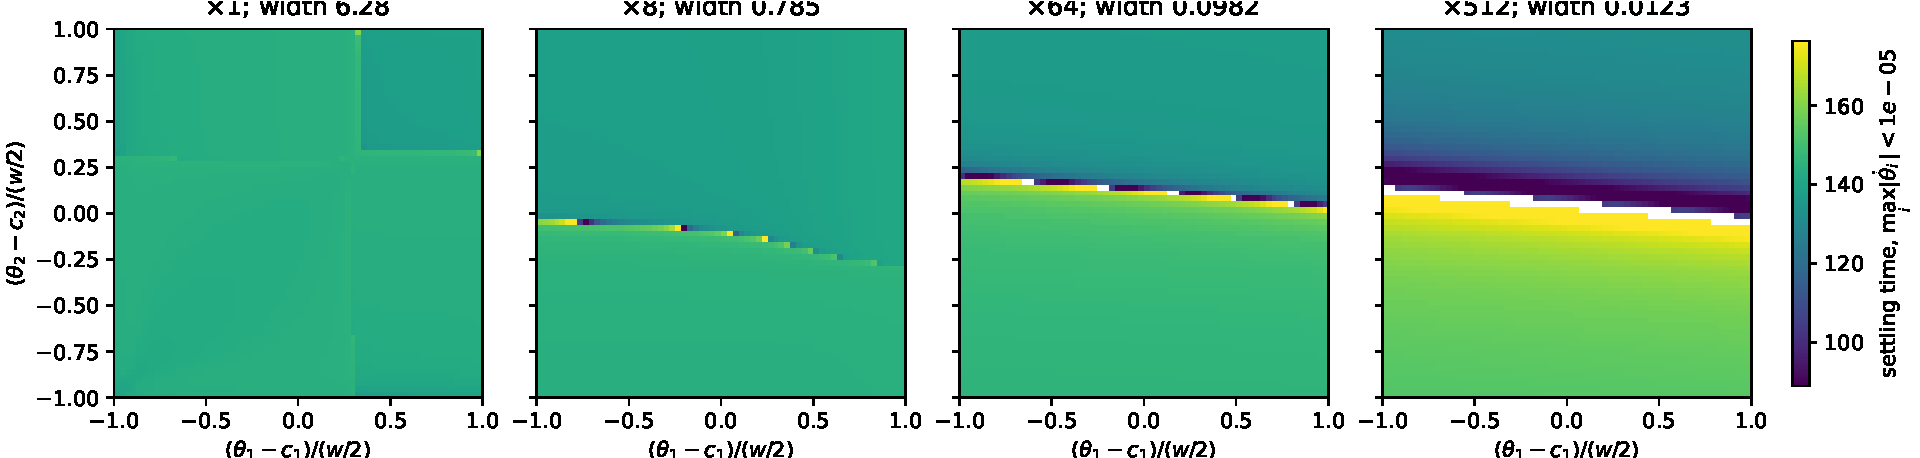
\includegraphics[width=\textwidth]{../../../data/spectral_self_attention/fractal_settling_atlas/fractal_settling_atlas.pdf}
\caption{Finite-horizon settling-time atlas at four adaptively selected
magnifications.  The first two initial angles vary and the third is fixed; axes are
normalized separately in each window.  White pixels fail the speed-and-tail
criterion by time 220.  Beyond the base view, the transition remains a single strip
at the displayed resolutions.}
\label{fig:settling-atlas}
\end{figure}

\begin{figure}[t]
\centering
\begin{subfigure}[t]{0.49\textwidth}
  \centering
  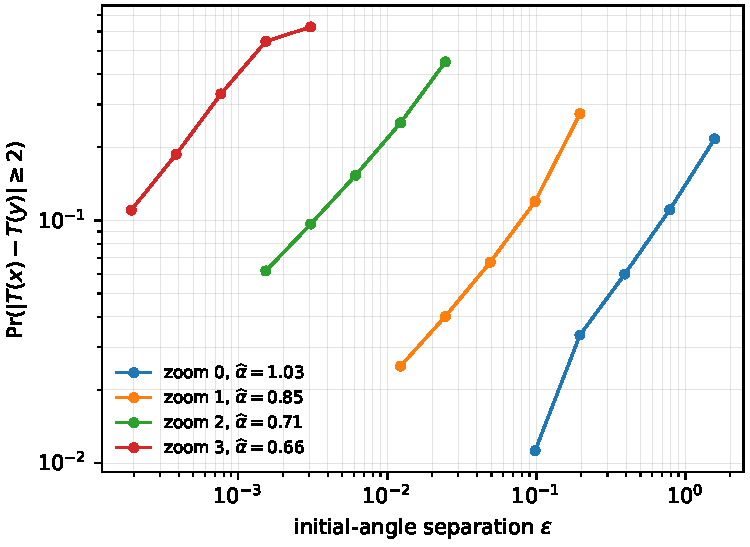
\includegraphics[width=\textwidth]{../../../data/spectral_self_attention/fractal_settling_atlas/fractal_settling_uncertainty.pdf}
  \caption{Measured statistic at $\delta=2$.}
\end{subfigure}\hfill
\begin{subfigure}[t]{0.49\textwidth}
  \centering
  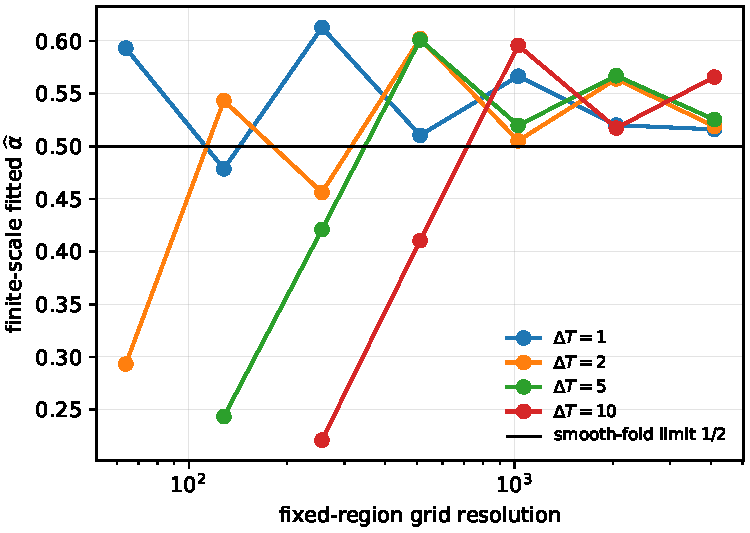
\includegraphics[width=\textwidth]{../../../data/spectral_self_attention/fractal_settling_atlas/fold_normal_form_null.pdf}
  \caption{Smooth critical-fold null.}
\end{subfigure}
\caption{Left: finite-scale power-law fits drift from $1.03$ to $0.66$ under
co-moving zoom.  Right: the nonfractal normal form
$\dot u=-4.761129215u^2$ approaches the analytic exponent $1/2$ under fixed-window
resolution refinement.  These regressions describe sampled scales; they are not
fractal-dimension estimates.}
\label{fig:settling-uncertainty-null}
\end{figure}

The experiment therefore does not exhibit an analogous fractal settling-time map in
this parameter slice.  It reproduces the visual fact that nearby starts can have
substantially different stopping times.  Their retained quiet finite-horizon endpoints
are consistent with approach to the same stable consensus.  At the tested scales,
the observed structure is quantitatively consistent with critical slowing near a
smooth saddle--node; neither the map geometry nor the three-trajectory tangent audit
provides evidence of a chaotic saddle.

\subsection{A rotating cluster from two head outputs}

Consider two planar heads with the same score $S=I$ and outputs $C_1=I$ and
$C_2=\omega J$, where $J$ rotates a vector by $\pi/2$.

\begin{proposition}[Exact multihead rotating consensus]
\label{prop:multihead-rotation}
For $\omega\ne0$, the synchronized manifold
$x_1=\cdots=x_n=x(\theta)$ is a periodic orbit with
$\dot\theta=\omega$ and period $2\pi/|\omega|$.  The collective exponent is zero and
all transverse exponents are $-1$.
\end{proposition}

\begin{proof}
At synchrony every row of each attention matrix is uniform, and the summed output is
$x(\theta)+\omega Jx(\theta)$.  Projection removes the first term.  If
$\theta_i=\theta+\eta_i$, then
$x_i^{\T}x_j=1+O((\eta_i-\eta_j)^2)$, so the attention weights have no first-order
variation.  The linearized phase equation is
$\dot\eta_i=\bar\eta-\eta_i$.  It has one zero collective rate and rate $-1$ on the
zero-mean subspace.
\end{proof}

With $\omega=0.8$ and 64 tokens, the simulation measures synchronization increasing
from $0.471$ to $1.000$ and angular speed $0.800000$.  This probes the larger basin of
the exact orbit.  Its Gram matrix is constant: the score kernel records no motion
although the transported values rotate.  Since the two heads share the same score,
their sum is algebraically one head with effective output $I+\omega J$; the example
proves stable rotation of summed outputs, not an irreducible effect of distinct
attention kernels.

\section{High dimension: orthogonality without decoupling}
\label{sec:dimension}

For two random unit directions in dimension $d$,
\[
 \mathbb E|x^{\T}y|\simeq\sqrt{\frac{2}{\pi d}}.
\]
With 24 tokens, six random heads, and 96 repetitions per dimension, mean absolute
token similarity falls from $0.638$ in dimension 2 to $0.050$ in dimension 256. Mean
similarity between head forces falls from $1.000$ to $0.049$. Independent heads
therefore combine almost like perpendicular directions.

Their scores also become similar. For fixed $\beta=3$, the effective number of
attended tokens out of 24 rises from $11.6$ to $23.6$. The dynamics does not split
into 24 independent systems; it retains an almost uniform global mean.

If $S=I$, the self-score remains one while cross-scores tend to zero. The limiting
self-weight is
\begin{equation}
 a_{ii}\longrightarrow\frac{\e^{\beta}}{\e^{\beta}+n-1}.\label{eq:self-mass}
\end{equation}
Thus $\beta$ must be appreciably larger than $\log n$ for genuine self-decoupling.
In the experiment's Wigner ensemble
$S=(G+G^{\T})/\sqrt{2d}$, cross-scores are $O(d^{-1/2})$; retaining nontrivial logits
therefore requires $\beta/\sqrt d$ to remain of constant order, rather than tend to
zero.  This scaling is tied to that ensemble.

In a practical Transformer, division by $\sqrt{d_{\mathrm{head}}}$ and learned query
and key norms are specifically chosen to keep logits of order one. Raw orthogonality of
embeddings is therefore insufficient to predict decoupling in a trained network.

Gao, Yang, and Chen obtain the complementary high-dimensional regime
\cite{gao2026clustered}.  Their tokens have norm $\sqrt d$, self-edges are masked,
$S=V=I$, and the logits use the standard $1/\sqrt d$ factor.  If within-cluster
overlaps exceed every cross-cluster overlap by a fixed gap $\Delta_a$, the leakage
from a cluster of size $n_a$ is exponentially small when
\begin{equation}
 \beta\sqrt d\,\Delta_a-\log\frac{n-n_a}{n_a-1}\longrightarrow+\infty.
 \label{eq:gao-gap}
\end{equation}
Their limiting clustered manifolds are normally attracting in internal directions;
collective rotations are neutral, and finite systems can coarsen on longer scales.
Our fixed-unit-norm, fixed-$\beta$ experiment instead sends cross-logit differences to
zero and therefore approaches uniform weights.  The conclusions differ because the
logit gap is $O(\sqrt d)$ in \eqref{eq:gao-gap} and $O(d^{-1/2})$ in our Wigner-score
control.

In the low-temperature mean-field limit, Alcalde, Bungert, Riedl, and Roith prove a
finite-time concentration estimate under invertibility of $S$ and symmetry plus a
spectral gap for $VS^{\T}$ \cite{alcalde2026concentration}.  Up to times of order
$\log\beta$, the selected subspace is controlled by the top eigenspace of
$VS^{\T}$; their later numerical phase is controlled by the spectrum of $V$.  This
gives one rigorous setting in which score--value selection and terminal value
transport occur on distinct time scales.  The symmetry of $VS^{\T}$ excludes the
circulating examples studied below.

\section{Many-token limit}
\label{sec:meanfield}

Define the empirical measure
\[
 \mu_t^n=\frac1n\sum_{i=1}^n\delta_{x_i(t)}.
\]
For a positive kernel $g$ and normalized attention, the velocity at $x$ is
\begin{equation}
 v_g[\mu](x)=P_x^{\perp}
 \frac{\int g(x^{\T}Sy)Vy\,d\mu(y)}
 {\int g(x^{\T}Sy)\,d\mu(y)}+P_x^{\perp}M(x).\label{eq:mean-field-velocity}
\end{equation}
Assume $g\in C^1$ is strictly positive on
$[-\norm{S}_{\mathrm{op}},\norm{S}_{\mathrm{op}}]$ and that $M$ is Lipschitz on the
sphere.  The denominator is then uniformly bounded away from zero, and
$v_g[\mu](x)$ is Lipschitz jointly in $x$ and in $\mu$ for the $1$-Wasserstein
distance.  The continuum equation is
\begin{equation}
 \partial_t\mu_t+\operatorname{div}_{\sphere}
 \bigl(\mu_t v_g[\mu_t]\bigr)=0.\label{eq:transport}
\end{equation}
The empirical measure of the $n$-token ODE is an exact atomic weak solution of this
equation.  The characteristic stability estimate gives, on every fixed time interval,
\begin{equation}
 W_1(\mu_t^n,\mu_t)\leq \e^{Ct}W_1(\mu_0^n,\mu_0),
 \label{eq:dobrushin}
\end{equation}
where $C$ depends on the fixed kernel, matrices, MLP, and interval.  Thus convergence
of the initial empirical measures implies the many-token limit.  This is the standard
Dobrushin argument for Lipschitz mean-field transport
\cite{dobrushin1979vlasov}; Transformer-specific transport formulations are developed
by Rigollet and by Castin, Ablin, Carrillo, and Peyr\'e
\cite{rigollet2025meanfield,castin2025unified}.

In our static quadrature control, a three-bump density is sampled and compared with an
8,192-point reference. The velocity error decays as $n^{-0.494}$, consistent with the
$n^{-1/2}$ Monte Carlo fluctuation: $0.289$ at 16 tokens, $0.146$ at 64, $0.071$ at
256, and $0.038$ at 1,024.  This measured exponent concerns one field evaluation; the
dynamical convergence statement is \eqref{eq:dobrushin}.

The deterministic drift limit used here scales both residual branches as $h$ and
keeps their weights fixed over depth.  Agazzi, Bruno, Mosig Garc\'ia, Saviozzi, and
Romito analyze the same serial order---attention, sphere normalization, one-hidden-
layer MLP, sphere normalization---with fresh independent MLP weights at every layer
and MLP residual scale $\sqrt h$ \cite{agazzi2026stochastic}.  They prove convergence
to a common-noise interacting diffusion, the associated stochastic transport
equation, propagation of chaos, and synchronization under a coercivity condition on
the noise.  Thus random MLP weights in that scaling do not reduce to the deterministic
field $M$ in \eqref{eq:mean-field-velocity}; the common Brownian field can itself drive
synchronization.

\subsection{Polygons become masses}

A distribution concentrated at $q$ positions has the form
\[
 \mu=\sum_{a=1}^q p_a\delta_{w_a},\qquad p_a>0,\quad\sum_a p_a=1.
\]
Set
\[
 Z_a=\sum_b p_b g(w_a^{\T}Sw_b).
\]
It is stationary exactly when
\begin{equation}
 P_{w_a}^{\perp}
 \left\{\frac{1}{Z_a}\sum_b p_b g(w_a^{\T}Sw_b)Vw_b
 +M(w_a)\right\}=0
 \quad\text{for every }a.\label{eq:atomic-equilibrium}
\end{equation}
Equivalently, the expression inside the projection can be multiplied by $Z_a$, in
which case the MLP contribution is $Z_aM(w_a)$.  Omitting this factor would change
the balance between attention and the MLP.
Integer token counts at each vertex therefore become real masses. Passing to the
integral enlarges the family because mass ratios need no longer be rational.

\begin{figure}[t]
\centering
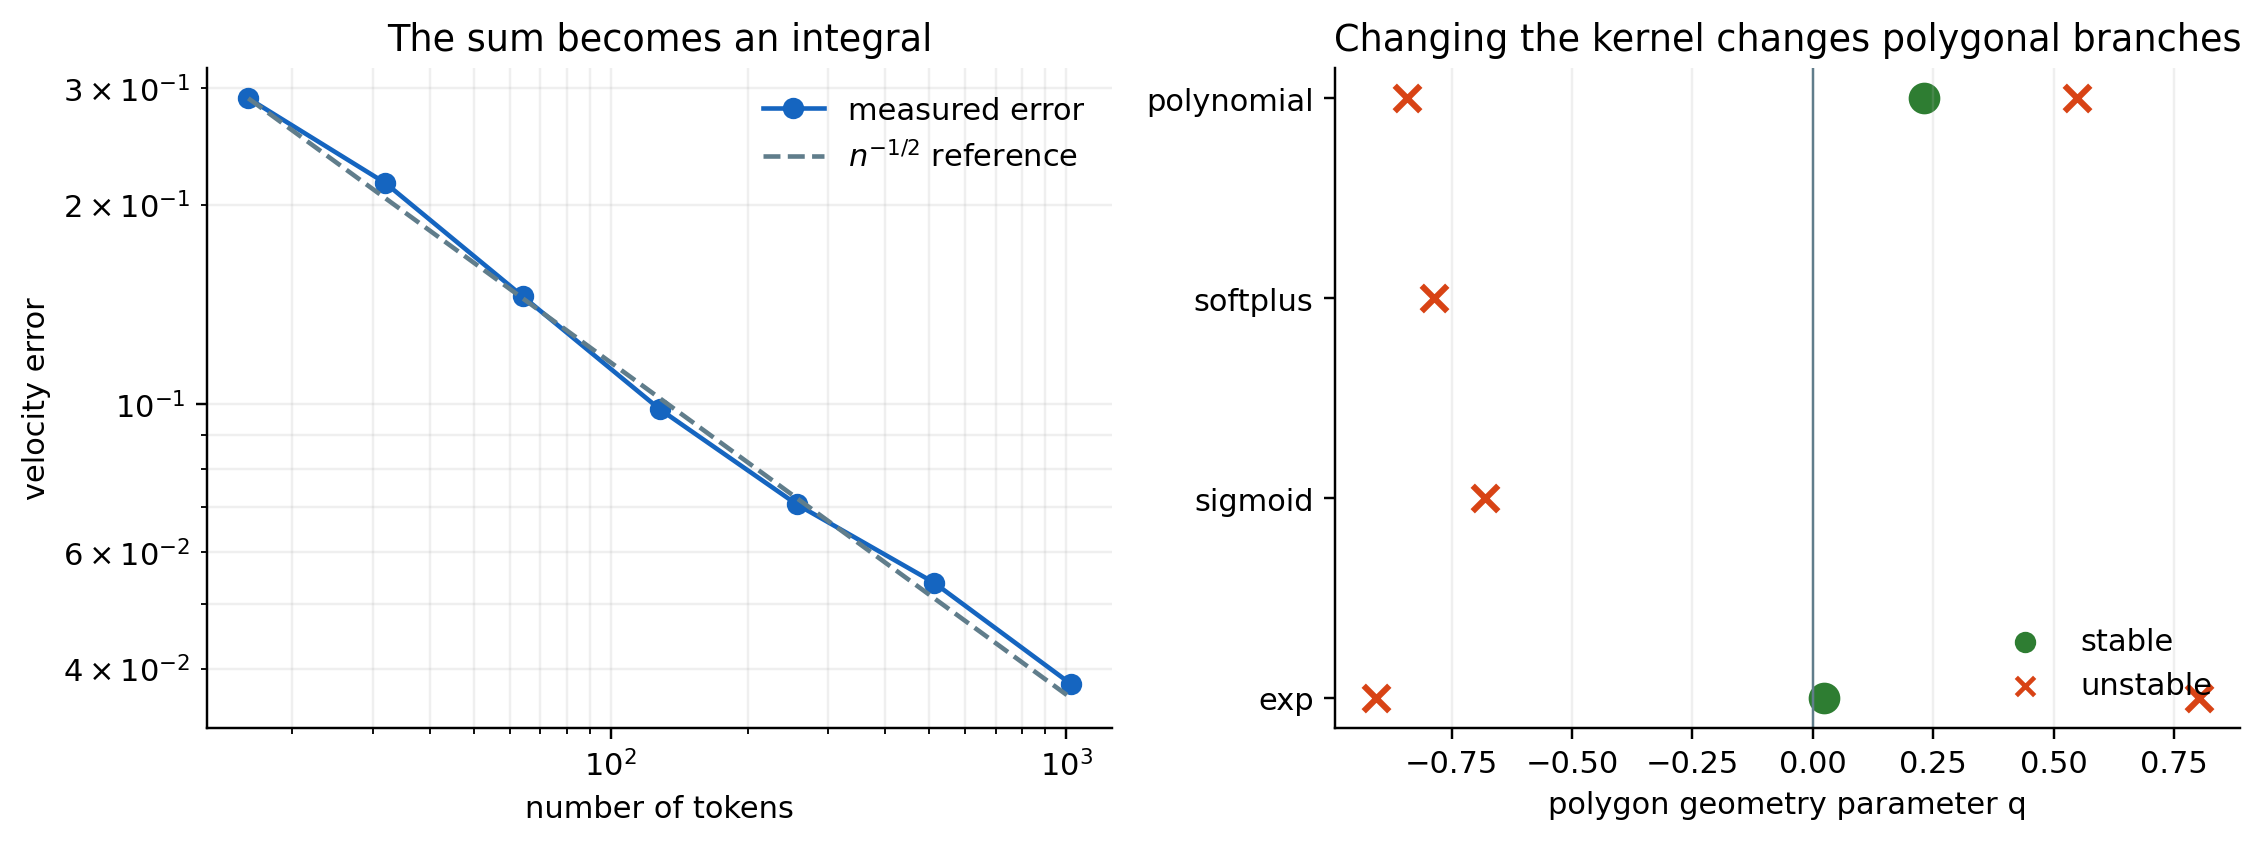
\includegraphics[width=\textwidth]{figures_en/meanfield_and_kernels.png}
\caption{Left: convergence of the token sum to the integral. Right: polygonal
positions found for four kernels; a green circle denotes a stable branch and an
orange cross an unstable one.}
\label{fig:meanfield-kernels}
\end{figure}

\subsection{Wasserstein geometry}

Wasserstein distance measures the minimum cost of moving one mass cloud into another.
It is naturally suited to \eqref{eq:transport}. It does not automatically turn every
attention system into energy descent.  Under the tied condition
$S=V=V^{\T}$, an antiderivative $G$ of $g$ gives the interaction energy
\[
 \mathcal E_G(\mu)=\frac12\iint G(x^{\T}Vy)\,d\mu(x)d\mu(y).
\]
Unnormalized attention is its projected gradient.  If $g>0$, row normalization
multiplies each token gradient by the positive mobility $1/Z_\mu(x)$, so the same
energy remains monotone. Untied or antisymmetric matrices can remove every common
energy.

\section{Changing the exponential or normalization}
\label{sec:kernels}

For $V=\operatorname{diag}(2,-3)$ and three equal masses, the four tested kernels are
\[
 g_{\exp}(s)=\e^{1.5s},\qquad
 g_{\rm sig}(s)=\frac{2}{1+\e^{-1.5s}},\qquad
 g_{\rm sp}(s)=\frac{\log(1+\e^{1.5s})}{\log 2},\qquad
 g_{\rm poly}(s)=\left(1+\frac{s}{3.01}\right)^4.
\]
The score interval is $[-3,3]$, so each kernel is strictly positive there and is
normalized to equal one at zero.
\begin{center}
\begin{tabularx}{0.88\textwidth}{YYl}
\toprule
Kernel & mixed three-group roots $q$ & stable root \\
\midrule
exponential & $-0.907,\ 0.024,\ 0.801$ & $0.024$ \\
bounded sigmoid & $-0.680$ & none \\
softplus & $-0.787$ & none \\
polynomial $(1+s/3.01)^4$ & $-0.842,\ 0.231,\ 0.548$ & $0.231$ \\
\bottomrule
\end{tabularx}
\end{center}

Mixed three-group branches also exist for the other kernels, with different locations and
stability.  In the attention-only equation, removing the denominator for a positive
kernel preserves the equilibrium equation token by token.  It preserves full
trajectories up to a single time reparametrization only when one token moves or when
all row denominators agree along the orbit.  For several moving tokens, the row
factors can change paths and basins.  In the presence of an MLP, several heads, or any
other additive field, the denominator can also move equilibria by changing the
relative strengths of the summed terms.

At a common attention-only equilibrium, the two Jacobians satisfy
\[
 J_{\rm unnorm}=\operatorname{Diag}(Z_i I_{d-1})J_{\rm norm},
\]
because the derivative of $Z_i$ multiplies a vanishing tangent field.  In the tied
gradient case, positive mobility preserves the Morse index of a hyperbolic critical
point.  For untied $S,V$, left multiplication by unequal positive row factors need
not preserve eigenvalue real parts, so local stability can also change.

Removing the sphere is much more radical.  For a single token initialized at unit norm
on the eigendirection of eigenvalue 2, spherical projection removes the whole push.
Without that projection, normalized attention gives $r'=2r$, so the norm reaches 10
at time $\log(10)/2=1.151\ldots$.  Removing the attention denominator as well gives
$r'=2r\exp(3r^2)$ under the tested exponential parametrization.  Its exact blow-up
time is
\[
 \int_1^\infty\frac{dr}{2r\exp(3r^2)}=\frac14 E_1(3)
 =0.003262\ldots .
\]
A radial push that was invisible on the sphere then controls the norm dynamics.

\section{State variables and observables}
\label{sec:observable}

Attention weights alone do not describe the state. For each head, velocity depends on
the two functions
\begin{equation}
 Z_\ell^{\mu}(x)=\int k_\ell(x,y)d\mu(y),\qquad
 N_\ell^{\mu}(x)=\int k_\ell(x,y)C_\ell y\,d\mu(y).\label{eq:observables}
\end{equation}
Head $\ell$ uses $N_\ell/Z_\ell$. One must therefore observe both who is selected and what is
transported. With a quadratic MLP, one must also retain the hidden measurements
$u_r^{\T}x_i+c_r$ and the linear projections used at the output.

For the aligned symmetric case, $H=XVX^{\T}$ and its pieces within each eigenspace
give a closed description up to rotations that commute with $V$.  In the general
anisotropic case, $XX^{\T}$ loses the orientation of the tokens relative to
$S,V$, and the MLP weights.  The following observables determine the instantaneous
velocity; no minimality or autonomous-closure claim is made:
\begin{enumerate}
  \item the full oriented token matrix $X$ (a Gram matrix alone is insufficient);
  \item the score matrices and weights of each head;
  \item directions after value and output transport;
  \item hidden MLP features;
  \item for a supervised task, positions, labels, and the readout.
\end{enumerate}

For the exponential kernel with symmetric positive-semidefinite $S$, the scalar score
kernel has the feature expansion
\begin{equation}
 \e^{\beta x^{\T}Sy}
 =\sum_{q=0}^{\infty}\frac{\beta^q}{q!}
 \left\langle(S^{1/2}x)^{\otimes q},(S^{1/2}y)^{\otimes q}\right\rangle .
 \label{eq:exponential-features}
\end{equation}
Thus $Z_\ell^\mu$ is a scalar kernel mean and $N_\ell^\mu$ is its
value-weighted, vector-valued analogue.  The latter cannot be reconstructed from
attention weights alone.  If $S$ is indefinite or nonsymmetric, a single
positive-definite feature map need not exist; the paired query and key maps, together
with the value attached to the same token, remain sufficient.

The hyperchaotic example makes this measurable: the maximum temporal standard
deviation of the weights is only $0.0034$, whereas that of the Gram geometry is
$0.481$. In the uniform-attention example, weight distance is exactly zero at every
step even when geometric distance is not.

\section{Training-time control and weight spectra}
\label{sec:training}

Isobe, Inoue, and Imaizumi fix unnormalized symmetric attention, add noise, and train
only an FFN that is linear in its parameters under a quadratic cost
\cite{isobe2026training}. Their optimal solution has three phases: tokens cluster,
remain near a well for a long time, and then the FFN acts strongly near the output to
reduce terminal loss. Their attention is parallel to the FFN in the continuous
equation, whereas our MLP is serial in the finite layer. \Cref{sec:model} explains why
the two models agree to first order and differ layer by layer at finite step size.

\subsection{Trained control around a polygon}

We train a small angular control, linear in five Fourier features, to move a stable
polygon toward a target rotated by $0.9$ radians. Maximum control in the first half is
$0.0011$; in the last five intervals it reaches $2.19$. Terminal error is $0.00133$.
The force is therefore about 2,000 times larger at the end than at the beginning.
The same late-control profile occurs in this polygon experiment.

\begin{figure}[t]
\centering
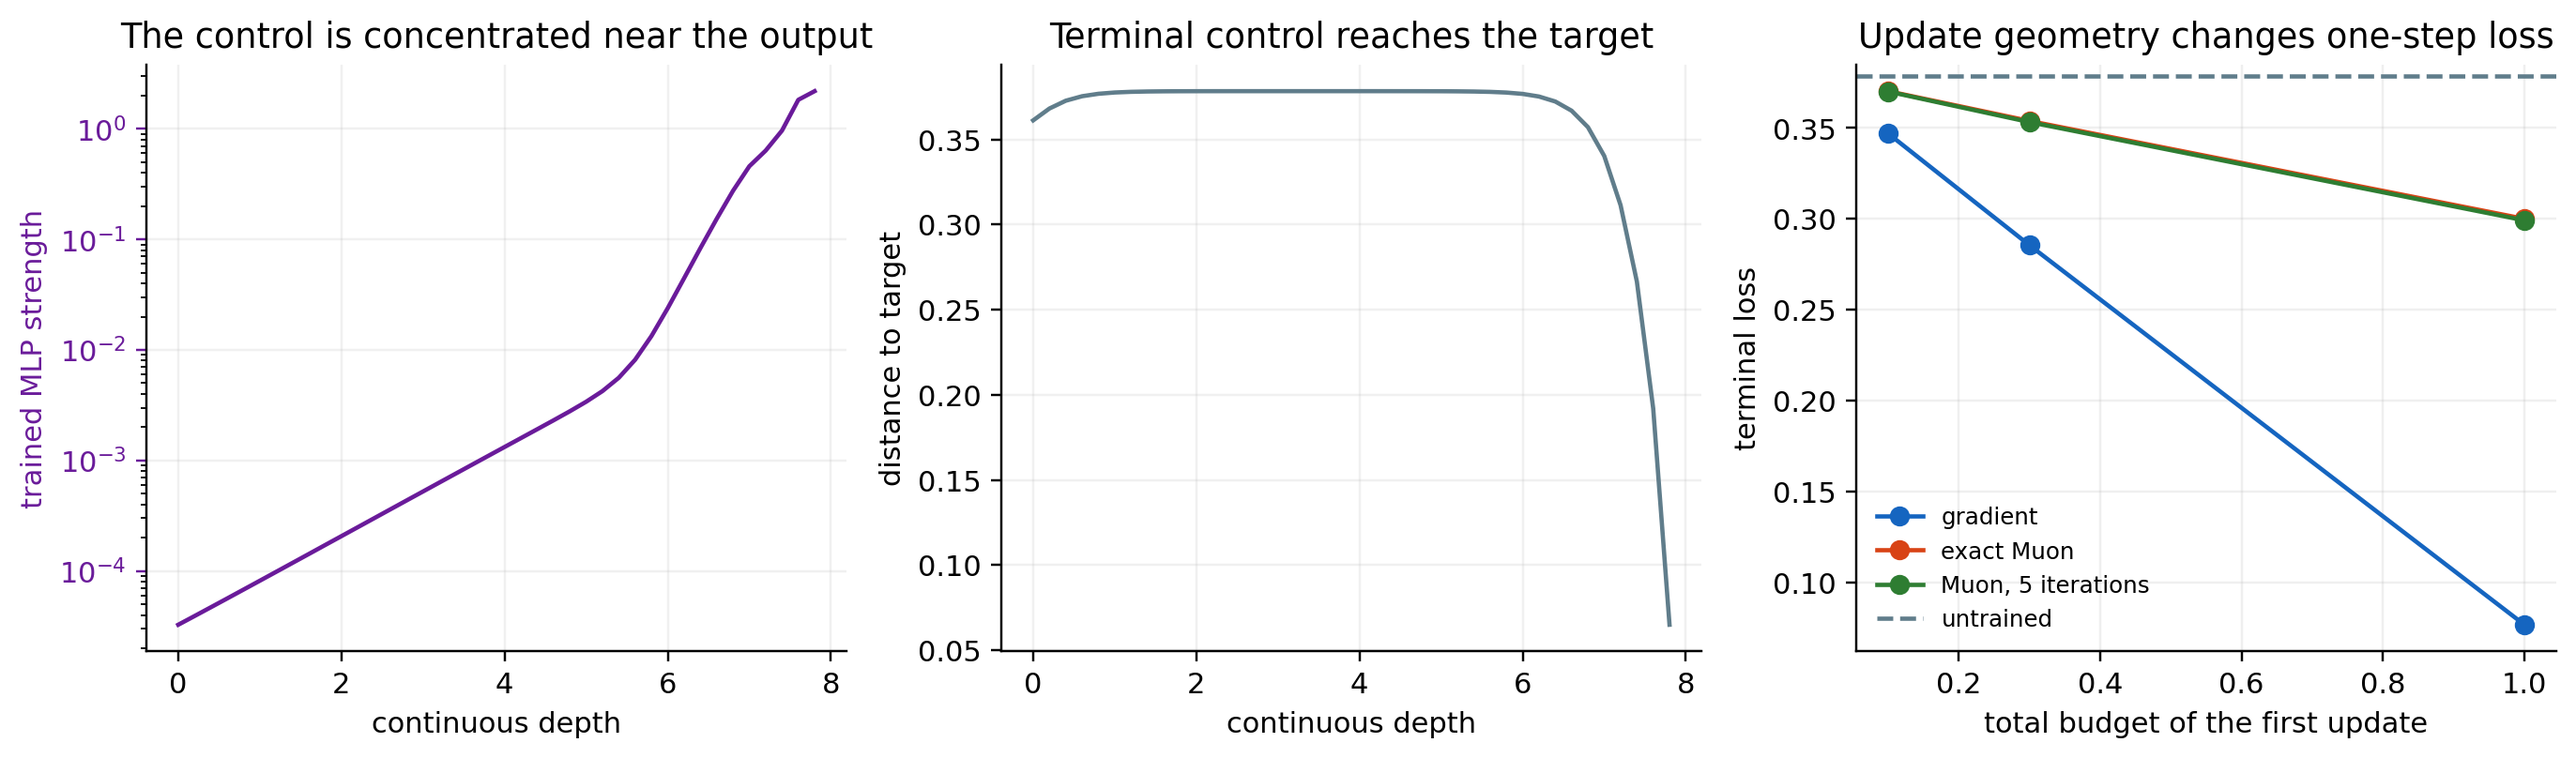
\includegraphics[width=\textwidth]{figures_en/training_and_muon.png}
\caption{Left: norm of the trained MLP control along continuous depth. Center:
distance to the rotated target. Right: terminal loss after one update at equal global
norm for gradient descent, exact Muon, and five Newton--Schulz iterations.}
\label{fig:training-muon}
\end{figure}

This result suggests a design principle: fix an attention dynamics that creates useful
basins, then train a serial MLP to remain in a basin, leave it, or move its destination.
It does not guarantee that every algebraic condition can be encoded by a small MLP or
that training globally finds the correct weights.

\subsection{Neural quadratic forms near initialization}

The preceding sections evolve token states with fixed weights.  The neural
quadratic-form (NQF) theory of Liu, Xu, Poggio, and Chuang concerns the evolution of
the weights during training \cite{ziyin2026nqf}.  The distinction matters because the
two problems have different state spaces and different spectra.

Let $W=(w_1,\ldots,w_r)\in\R^{p\times r}$ collect $r$ exchangeable components of a
scalar module evaluated on an input $\xi$.  Under three-times differentiability,
permutation symmetry of the components, and zero component gradient when that
component is zero, their theorem gives
\begin{equation}
 f_\xi(W)=f_\xi(0)+\operatorname{Tr}\!\left(\mathcal M_W A(\xi)\right)
 +O(\norm{W}^3),\qquad
 \mathcal M_W=WW^{\T}\succeq0,
 \label{eq:nqf}
\end{equation}
where the symmetric structure matrix $A(\xi)\in\R^{p\times p}$ is determined by the
architecture and the input.  This statement applies to a factorized parameterization
whose exchangeable components satisfy the hypotheses.  Training the effective
matrices $S$ and $V$ directly introduces linear parameter sectors and is a different
model.  Residual sphere normalization is smooth around a unit base token:
$\mathcal N(x+\delta)=x+P_x^\perp\delta+O(\norm{\delta}^2)$.  It therefore projects
the leading structure matrix as long as the pre-normalization vector stays nonzero;
a nonresidual normalization at the origin would require a separate analysis.

For attention, the order at which a parameter appears depends on what is trained.
Let $X_c\in\R^{d\times n}$ be a context matrix, with
$\bar x=X_c\one/n$ and
$\Sigma_{X_c}=X_cX_c^{\T}/n-\bar x\bar x^{\T}$.  Put
$Q=\varepsilon\widehat Q$, $K=\varepsilon\widehat K$,
$V=\varepsilon\widehat V$, and $o=\varepsilon\widehat o$.  Direct softmax expansion
at inverse temperature $\beta$ gives
\begin{equation}
 f_{\rm full}(\varepsilon)
 =\varepsilon^2\widehat o^{\T}\widehat V\bar x
 +\frac{\beta\varepsilon^4}{\sqrt{d_k}}\widehat o^{\T}\widehat V
 \Sigma_{X_c}\widehat K^{\T}\widehat Qx+O(\varepsilon^6).
 \label{eq:full-attention-expansion}
\end{equation}
Thus value--readout learning is quadratic, while query--key routing first enters at
quartic order.  The quadratic full-head structure matrix has a bipartite
value--readout block, hence paired positive and negative eigenvalues, together with a
large zero sector containing the query and key directions.  If the value and readout
are fixed and merged into $c$, training only
$Q$ and $K$ instead gives
\begin{equation}
 f_{QK}(\varepsilon)=c^{\T}\bar x+
 \frac{\beta\varepsilon^2}{\sqrt{d_k}}
 (\Sigma_{X_c}c)^{\T}\widehat K^{\T}\widehat Qx+O(\varepsilon^4).
 \label{eq:qk-attention-expansion}
\end{equation}
Under column-wise vectorization, the corresponding structure matrix has the
off-diagonal block
\[
 \frac{\beta}{2\sqrt{d_k}}
 \bigl[x(\Sigma_{X_c}c)^{\T}\bigr]\otimes I_{d_k},
\]
with its transpose in the opposite block.  A different vectorization permutes rows
and columns.  The spectral experiment below sets $\beta=1$.

For mean-squared loss on samples $(\xi_\mu,y_\mu)$, the pure quadratic model has
\begin{align}
 \mathcal L(W)&=\frac1m\sum_{\mu=1}^m
 \left[\operatorname{Tr}(\mathcal M_WA_\mu)-y_\mu\right]^2,\\
 \dot W&=-\mathcal H_W W,\qquad
 \dot{\mathcal M}_W=-\mathcal H_W\mathcal M_W-\mathcal M_W\mathcal H_W,
 \label{eq:nqf-matrix-flow}\\
 \mathcal H_W&=\frac4m\sum_{\mu=1}^m
 \left[\operatorname{Tr}(\mathcal M_WA_\mu)-y_\mu\right]A_\mu .
\end{align}
If the $A_\mu$ commute, write
$A_\mu=P\operatorname{Diag}(\lambda_{\mu,1},\ldots,\lambda_{\mu,p})P^{\T}$ and
$z_k=(P^{\T}\mathcal M_WP)_{kk}$.  Then
\begin{equation}
 \dot z_k=\frac8m\left[
 \sum_\mu y_\mu\lambda_{\mu,k}
 -\sum_j\left(\sum_\mu\lambda_{\mu,k}\lambda_{\mu,j}\right)z_j
 \right]z_k.
 \label{eq:nqf-glv}
\end{equation}
This is the generalized Lotka--Volterra reduction proved in the NQF paper.

Equation \eqref{eq:nqf-glv} organizes every sign pattern at initialization.  With
\begin{equation}
 r_k=\frac8m\sum_\mu y_\mu\lambda_{\mu,k},
 \label{eq:nqf-growth}
\end{equation}
a mode with $r_k>0$ initially grows, a mode with $r_k<0$ initially decays, and a
zero-rate mode is decided by nonlinear coupling.  In a generic coupled
Lotka--Volterra system, later competition can suppress or delay a mode despite its
positive initial rate.

The logarithmic ignition formula requires one of the solvable reductions in the NQF
analysis: orthogonal features, or isotropic samples with $\mathcal M_W(0)$ and the
target operator simultaneously diagonalizable.  Let $\zeta_k>0$ denote the positive
target or generator coefficient in the convention of the corresponding reduction;
the linear growth exponent of $z_k$ is $a\zeta_k$, with $a=1$ for orthogonal features
and $a=2$ for isotropic samples.  If
$z_k(0)=\epsilon\rho_k$ with $\rho_k$ bounded above and below independently of
$\epsilon$, then
\begin{equation}
 t_k^\star=\frac1{a\zeta_k}\log\frac1\epsilon+O(1),
 \qquad
 a=\begin{cases}1,&\text{orthogonal features},\\2,&\text{isotropic samples}.
 \end{cases}
 \label{eq:nqf-ignition}
\end{equation}
Equal $\zeta_k$ have no separation proportional to $\log(1/\epsilon)$; distinct
positive rates do.  Here $\epsilon$ is the initial scale of an eigenvalue or diagonal
mode of $\mathcal M_W$.  If entries of $W$ instead have standard deviation $\sigma$,
then typically $\epsilon\propto r\sigma^2$, so the slope against
$\log(1/\sigma)$ is twice the slope in \eqref{eq:nqf-ignition}.
Gaussian and norm-fixed initializations change the $O(1)$ intercept through
$\rho_k$; they should leave the logarithmic slope unchanged in the quadratic
gradient-flow regime.  A normalization layer can change $A_\mu$ or violate the
smoothness assumptions, and Muon's polar update is not governed by
\eqref{eq:nqf-matrix-flow}.

There is a conditional link to inference-space bifurcations.  Suppose a scalar mode
$z_k$ in one of the solvable reductions parametrizes a frozen-weight equilibrium
branch, and a simple eigenvalue $\ell(z_k)$ of its token-state Jacobian satisfies
$\ell(z_c)=0$ and $\ell'(z_c)\ne0$ at a fixed threshold below the mode's plateau.
The training time at which that branch changes stability then obeys
\begin{equation}
 t_{\rm bif}=\frac{1}{a\zeta_k}\log\frac1\epsilon+O(1).
 \label{eq:nqf-bifurcation-clock}
\end{equation}
Two bifurcations controlled by distinct growth rates therefore acquire a separation
of order $\log(1/\epsilon)$; an exact rate degeneracy removes that leading
separation.  This implication requires an identified map from the NQF mode to the
state Jacobian.  Neither the NQF theorem nor the training experiment of Lai et al.
supplies that map for a general Transformer.

The saddle--node in \eqref{eq:fractal-consensus-field} gives a second conditional
case.  If a learned MLP multiplier satisfies
$\Gamma(t)=\Gamma_0+b_\Gamma z_k(t)$ with $b_\Gamma>0$, and the threshold
$z_c=(\gamma_c-\Gamma_0)/b_\Gamma$ is fixed independently of $\epsilon$ and satisfies
$0<z_c<z_{k,\infty}$, then the time at which the
synchronized pair is created still has the logarithmic form
$(a\zeta_k)^{-1}\log(1/\epsilon)+O(1)$.  The post-creation root separation and
Jacobian eigenvalue magnitude are both
$\Theta(\sqrt{\Gamma-\gamma_c})$; this is not the simple linear eigenvalue crossing
assumed in the preceding paragraph.  This is
an implication of the assumed scalar coupling, not a claim that generic Transformer
training follows that path.

The NQF scaling theorem additionally takes an infinite-mode limit and assumes
$\alpha_1>1$, $\alpha_2>0$, and controlled initial coefficients.  In the theorem,
the effective growth rates and target strengths have the exact tails
$\zeta_k=c_\zeta k^{-\alpha_2}$ and
$\mathcal V_k=c_{\mathcal V}k^{-\alpha_1}$.  If
$z_k(0)=\epsilon c_k k^{-b}$ with $c_k$ bounded above and below and
$b\geq\alpha_1-\alpha_2$, then, first taking the number of modes to infinity at
fixed $\epsilon$ and then taking $\epsilon\to0$, the excess loss at
$\tau=t/\log(1/\epsilon)$ scales as
\begin{equation}
 \mathcal E(\tau)=\Theta\!\left(
 \tau^{-(\alpha_1-1)/\alpha_2}\right).
 \label{eq:nqf-scaling}
\end{equation}
for almost every rescaled time $\tau$ in the theorem's domain.
The architecture determines the structure matrices; it does not imply these
power-law tails.

\subsection{Numerical spectral atlas}

We tested the preceding statements in the exactly solvable isotropic NQF, rather than
in a generic trained Transformer where the quadratic approximation would be local.
For every dimension $p\leq6$, the experiment enumerates every inertia and every
partition of the positive and negative eigenvalue multiplicities.  There are 280 such
categorical classes.  Continuous eigenvalue magnitudes are not enumerated.  Write
$\gamma_k$ for the eigenvalues of the symmetric label-weighted generator
$Y=4m^{-1}\sum_\mu y_\mu A_\mu$.  Across all classes, the maximum error between the
fitted initial rate of $\log z_k$ and the predicted value $2\gamma_k$ is
$1.23\times10^{-7}$.

Ignition was measured for generator eigenvalues $(1,0.7,0.7,0.25)$, widths 32, scales
$\epsilon=10^{-2},\ldots,10^{-8}$, and 64 paired replicates under Gaussian, row-norm-
fixed, and row-Stiefel initializations.  The largest relative error in the fitted
slopes of $t_k^\star$ against $\log(1/\epsilon)$ is $0.101\%$.  The two modes with
eigenvalue $0.7$ have a fitted difference slope of magnitude at most
$1.60\times10^{-4}$, consistent with the absence of logarithmic separation at an
exact degeneracy.  Initialization changes the intercept and its variance.  It does
not change the slope within this solvable regime.  Individual eigenvectors inside a
degenerate eigenspace are not identifiable, so their comparison uses projector
overlap; outside degeneracies, the leading eigendirections of $\mathcal M_W$ align
with those of the generator during growth.

The attention expansion gives a separate structural check.  For a random
five-dimensional context of length 11, key dimension 3, value dimension 4, and 48
samples, the full-head quadratic generator has inertia $(4,46,4)$: four positive,
46 zero, and four negative eigenvalues.  Removing softmax normalization preserves
that inertia and multiplies its spectral radius by 11 in this zeroth-order
value--readout sector.  With fixed values and readout, the $QK$ generator has inertia
$(15,0,15)$; positive and negative eigenvalues pair to within
$2.9\times10^{-15}$.  These are structure-matrix spectra at initialization, not the
eigenvalues of $V$ or a token-state Jacobian.

For the NQF tail assumptions, $16{,}384$ modes with
$(\alpha_1,\alpha_2)=(2,0.8)$ give a fitted excess-loss exponent $-1.25623$, compared
with the prediction $-1.25$.  Exponential-rate and flat-rate controls do not exhibit
the same stable power-law slope.  Finally, a spiked-Wishart control with aspect
$\gamma_{\rm asp}=p/r=1/2$ separates the BBP claim from the NQF dynamics.  Its
population spike satisfies $1+\theta(t)=\exp(2\delta t)$ with $\delta=0.25$, and hence
$t_c=\log(1+\sqrt{\gamma_{\rm asp}})/(2\delta)$.  At $p=256$, $r=512$, and 32
replicates, the null top eigenvalue is $2.8678$ versus the asymptotic bulk edge
$2.9142$, and its mean squared spike overlap is $0.00187$.  At twice the critical
time, the measured outlier is $3.6453$ versus $3.6754$, and the overlap is $0.6861$
versus $0.6847$.  A row-Stiefel initialization has
$\mathcal M_W(0)=\epsilon I$ and no finite-width Wishart bulk; its planted direction
is selected for every $t>0$ after anisotropic growth begins, although no direction is
distinguished at $t=0$.  The BBP transition is therefore initialization-ensemble
specific, whereas the logarithmic NQF clocks persist across the three tested
initializations.

\begin{figure}[t]
\centering
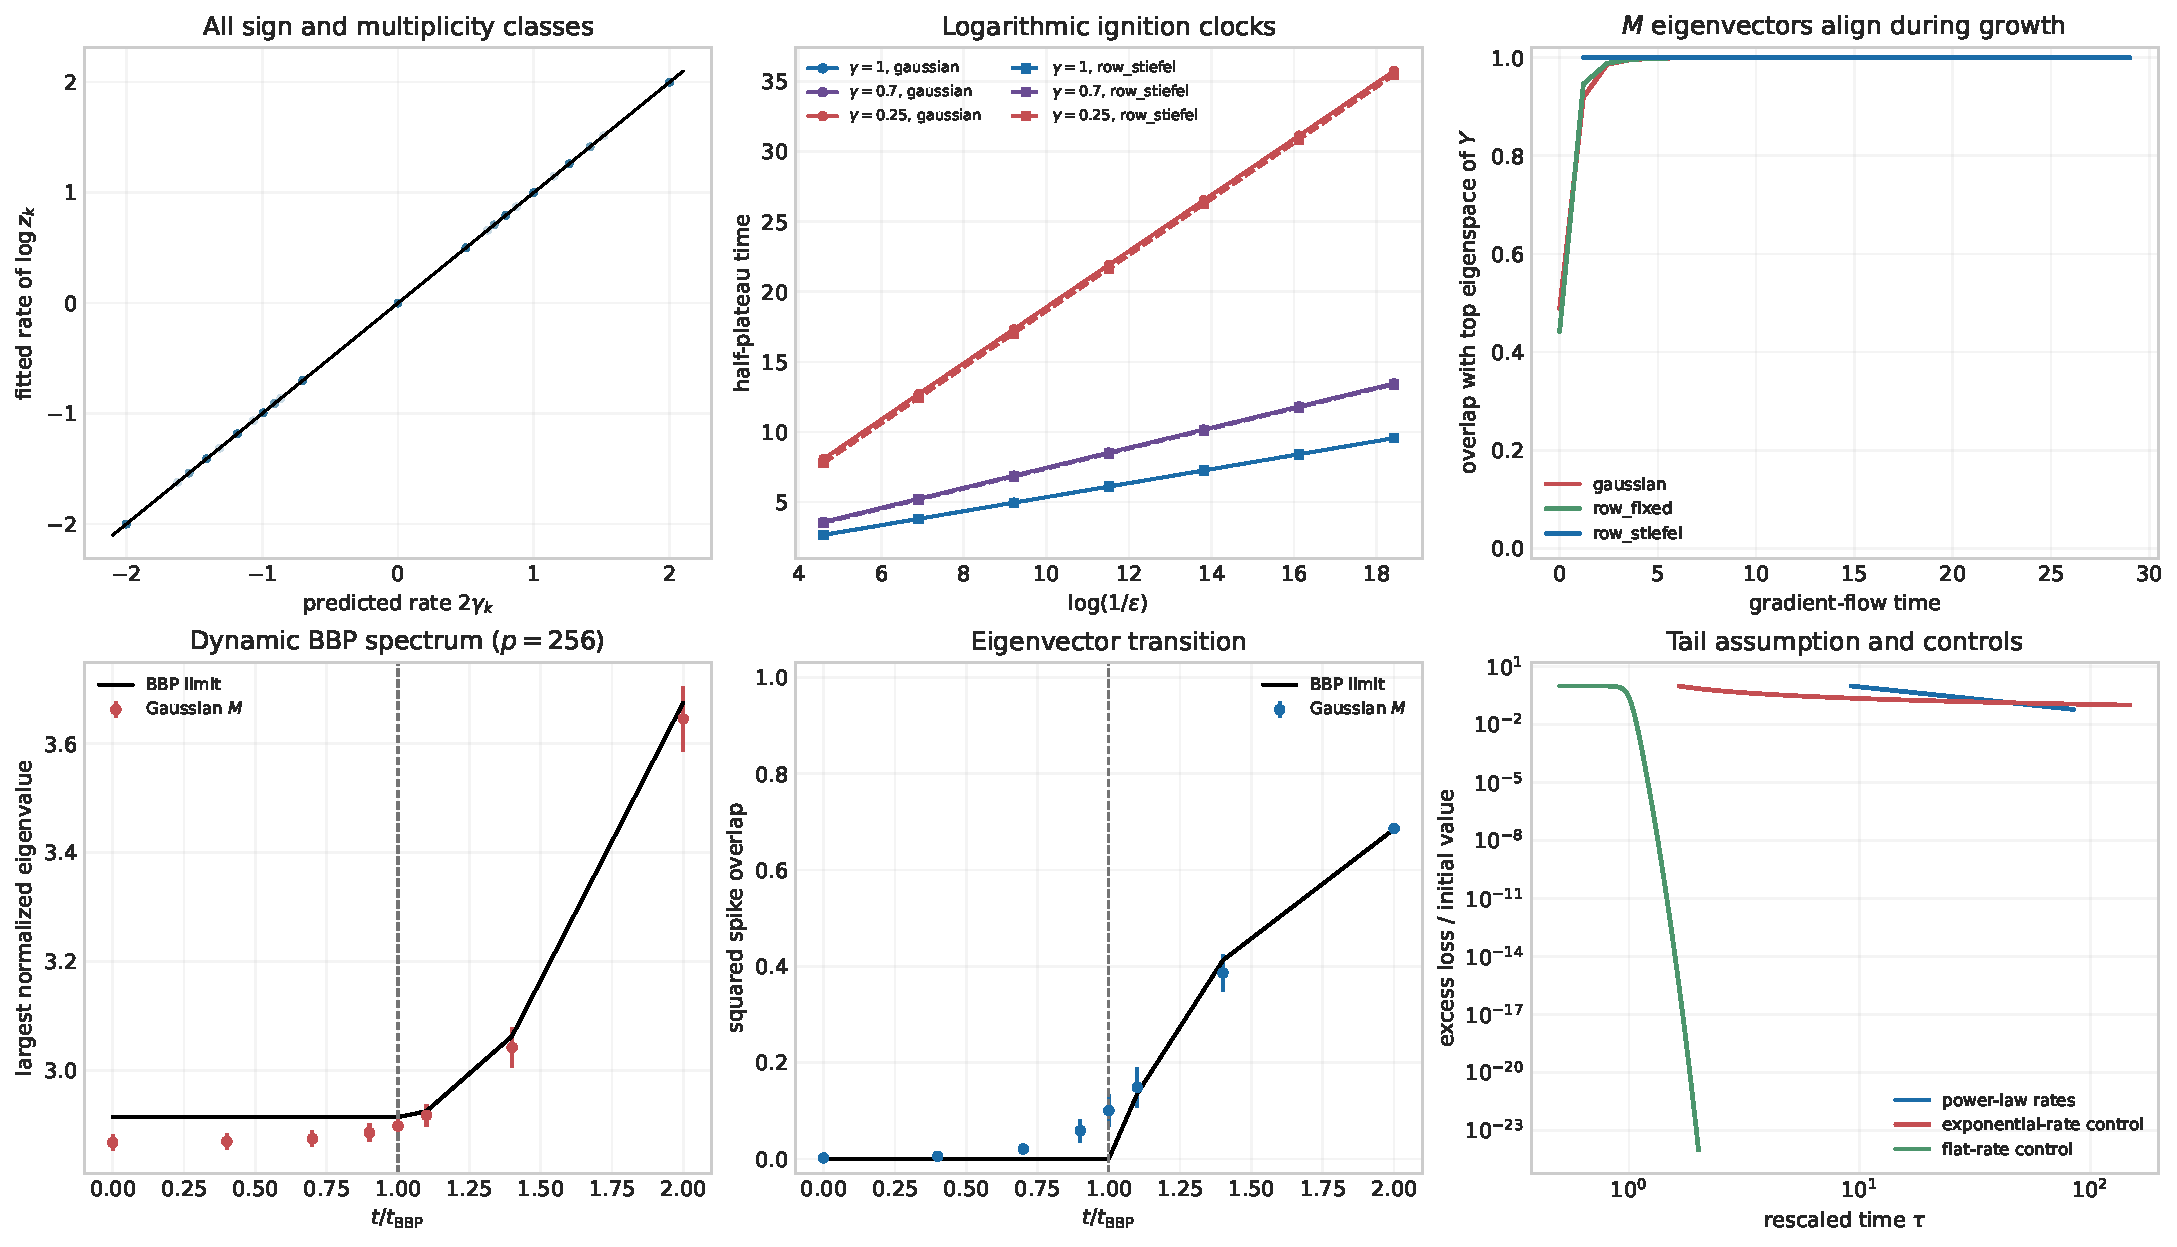
\includegraphics[width=\textwidth]{../../../data/spectral_self_attention/nqf_training_spectrum_atlas/nqf_training_spectrum_atlas.pdf}
\caption{Spectral audit of the solvable isotropic NQF.  Top row: predicted and fitted
initial mode rates over all 280 categorical spectra; ignition clocks for three
initializations; alignment of identifiable eigenspaces of $\mathcal M_W$ with the
generator.  Bottom row: top eigenvalue and spike overlap in the spiked-Wishart
control, followed by the power-law tail and two non-power-law controls.  Error bars
are standard errors over 32 Gaussian matrices in the $p=256$ BBP panels.}
\label{fig:nqf-atlas}
\end{figure}

\subsection{Three spectra that should not be identified}

The eigenvalues of $V$ in \cref{thm:spectral-gram} classify stationary token
geometry in the tied fixed-weight flow.  Eigenvalues of the tangent Jacobian and
Floquet or Lyapunov exponents determine inference-depth stability.  Eigenvalues of
$A_\mu$, $\mathcal H_W$, and $\mathcal M_W$ determine training-time parameter growth
in the NQF approximation.  No general identity relates these spectra.  An empirical
comparison must measure their eigenvector overlaps as well as their eigenvalues.

A Baik--Ben Arous--P\'ech\'e (BBP) outlier requires a further random-matrix model
\cite{baik2005phase,paul2007spiked}.  For the standard rank-one spiked covariance
control with aspect ratio $\gamma_{\rm asp}=p/r$ and population covariance
$I+\theta uu^{\T}$, the top sample eigenvalue separates from the Marchenko--Pastur
bulk only for $\theta>\sqrt{\gamma_{\rm asp}}$.  The limiting bulk edge is
$(1+\sqrt{\gamma_{\rm asp}})^2$, while the outlier limit is
$(1+\theta)(1+\gamma_{\rm asp}/\theta)$.  The low-dimensional $V$ spectra used for the
attractor examples have no bulk limit and admit no BBP interpretation.

\subsection{A first Muon step}

If the gradient of a matrix at depth $k$ is $G_k=U_k\Sigma_kR_k^{\T}$, a gradient
step is $-\alpha G_k$. An idealized Muon step instead uses
\begin{equation}
 -\eta U_kR_k^{\T}.\label{eq:muon}
\end{equation}
It preserves singular directions and equalizes nonzero magnitudes. At the first step
from zero momentum, momentum only changes the global gradient scale, which this polar
factor then removes.
Under an operator-norm constraint per matrix, this is the steepest direction; under
the $L^2$ constraint of Imaizumi's theorem, the gradient is naturally favored.

In our 40-slice analogue, the final gradient is $7.11\times10^{11}$ times larger than
the initial gradient. At total budget $0.3$, loss falls from $0.37839$ without training
to $0.28547$ with gradient descent, $0.35385$ with exact Muon, and $0.35323$ with five
Newton--Schulz iterations. At budget $1.0$, Muon acts much earlier and destroys the
plateau, while the gradient still concentrates its action on the last slice. This is
not a universal ranking: it shows that the norm used to compare updates determines
the winner.

Recent associative-memory analyses give another explanation for Muon's usefulness: it
balances learning of rare directions more evenly than anisotropic updates
\cite{wang2025muon,kim2026spectral}. Our experiment does not replace those results; it
shows their analogue along the depth of a polygonal dynamics.

\section{Slow Ornstein--Uhlenbeck weight dynamics}
\label{sec:ou}

Massucco and collaborators represent heads by a distribution of matrices that changes
with depth \cite{massucco2026time}. In their Ornstein--Uhlenbeck regime,
\begin{equation}
 d\Theta_t=\kappa(F-\Theta_t)dt+\sqrt{2\kappa}\,\sigma\,dB_t,
 \qquad \kappa>0,\label{eq:ou}
\end{equation}
the weight law returns at rate $\kappa$ to a Gaussian centered at $F$ with entrywise
stationary variance $\sigma^2$.  The simulator uses the exact transition
\[
 \Theta_{t+\Delta t}=F+\e^{-\kappa\Delta t}(\Theta_t-F)
 +\sigma\sqrt{1-\e^{-2\kappa\Delta t}}\,\Xi_t.
\]
At $\kappa=0$, it draws $\Theta_0=F+\sigma\Xi_0$ and freezes that draw.  Massucco and
collaborators prove asymptotic stationarity under compact parameter support and a
bound on accumulated explicit time variation of the energy.  A Gaussian OU path has
unbounded support and nonintegrable path variation, so that theorem does not establish
relaxation for the literal stochastic process above.  Their OU discussion gives a
formal finite-head/noise estimate and numerical evidence; it does not cover the slow
sample-path regime studied here.

Our first approach isolates renewal speed. It uses 32 tokens on $\sphere^2$, four
heads, 12 repetitions, $\sigma=0.65$, step $0.02$, and 2,000 steps. The target mean
matrix has eigenvalues $(1.2,1.0,0.2)$. The OU rate ranges from 0 to 10.

\begin{figure}[t]
\centering
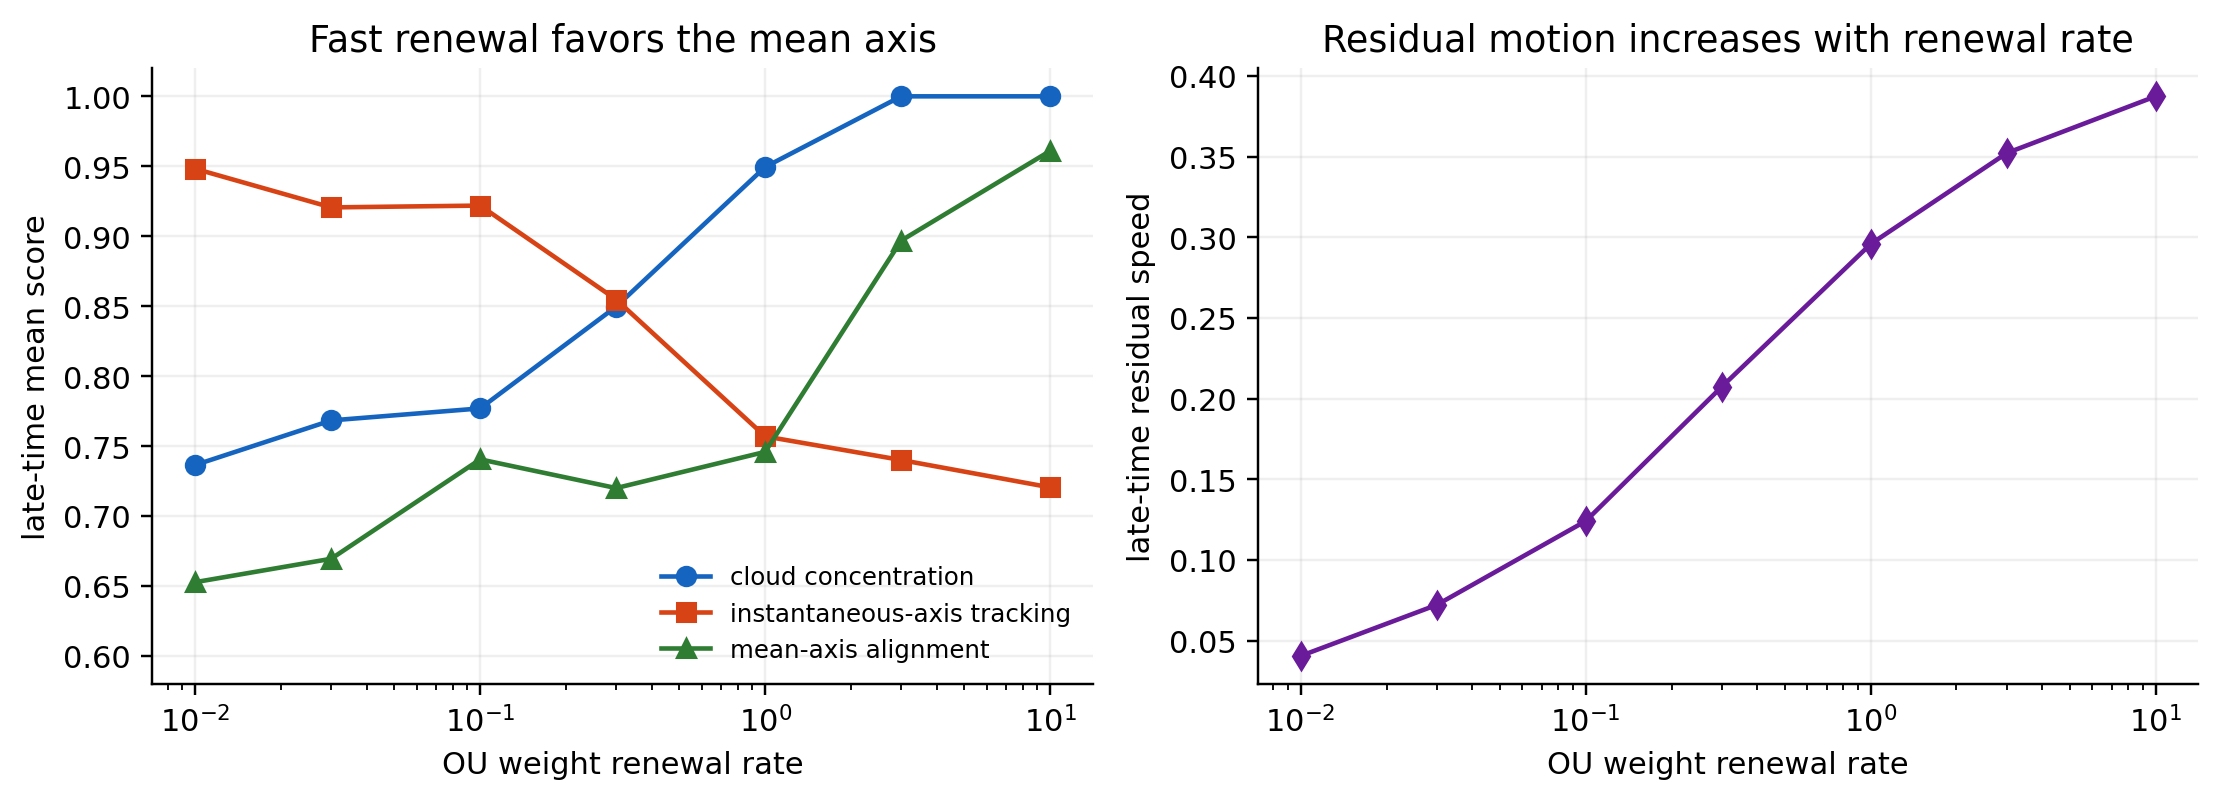
\includegraphics[width=0.88\textwidth]{figures_en/slow_ou.png}
\caption{Late-time statistics versus the OU renewal rate for 32 tokens, four heads,
12 repetitions, $\sigma=0.65$, and integration step $0.02$. Left: concentration and
alignment statistics. Right: residual token speed.}
\label{fig:slow-ou}
\end{figure}

At rate $0.01$, late concentration is $0.736$ and instantaneous-axis tracking is
$0.948$. At rate $0.3$, they are $0.850$ and $0.855$. At rate 3, concentration is
nearly one, but instantaneous tracking is only $0.740$, while mean-axis alignment is
$0.897$. Late speed grows from $0.040$ to $0.352$. This exposes three time scales:
token contraction, landscape motion, and noise averaging.

If the frozen system has a uniformly attracting equilibrium branch, with a relaxation
gap bounded away from zero and no nearby bifurcation, sufficiently slow weight motion
gives quasistatic tracking.  When relaxation and renewal times become comparable,
the numerical sweep exhibits lag and path dependence; basin changes can occur near a
stability boundary.  The sweep measures lag and concentration.  It does not establish
a chaotic attractor caused by slow OU weights.

The saddle--node in \eqref{eq:fractal-saddle-node-normal-form} quantifies the loss of
this separation.  With $\mu=\gamma-\gamma_c>0$, the stable-branch gap is
$\Theta(\sqrt\mu)$ and $|d\theta_\star/d\gamma|=\Theta(\mu^{-1/2})$.  For a smooth
deterministic parameter path, linear-response power counting gives a tracking lag of
order $|\dot\gamma|/\mu$.  Keeping this lag small relative to the branch separation
$\Theta(\sqrt\mu)$ requires
\begin{equation}
 |\dot\gamma|\ll \mu^{3/2}.
 \label{eq:saddle-adiabatic-condition}
\end{equation}
This condition necessarily fails in a shrinking neighborhood of the bifurcation for
any fixed nonzero sweep rate.  Brownian OU paths are not differentiable, so
\eqref{eq:saddle-adiabatic-condition} is not a samplewise criterion for
\eqref{eq:ou}.  Applying the scalar condition to matrix-valued OU dynamics would
also require identifying the coordinate of $\Theta_t$ that controls $\gamma$; the
corresponding noisy first-passage problem remains open here.

\section{Relations to statistical-physics models}
\label{sec:statphys}

For $\beta>0$, each softmax row is exactly a conditional Boltzmann law:
\[
 a_{ij}=\frac{\e^{-E_{ij}/T}}{\sum_k\e^{-E_{ik}/T}},
 \qquad E_{ij}=-x_i^{\T}Sx_j,\qquad T=1/\beta.
\]
Uniform attention at $\beta=0$ is the infinite-temperature limit.
This alone does not make the system equilibrium matter: the weights are Boltzmann
probabilities, but the token trajectory is deterministic. A genuine heat bath would
require tangent Brownian noise. If the field is a gradient and noise is matched to its
mobility, the stationary law is Gibbs. With antisymmetric transport or a general MLP,
currents can persist and the system remains out of equilibrium.

The tied isotropic choice $S=V=I$ is a mean-field $O(d)$ vector-spin model on the sphere with an
exponential ferromagnetic pair interaction, followed by deterministic zero-noise
gradient ascent with token-dependent mobility.  Several tied symmetric heads give a
sum of anisotropic vector-spin interactions only when their mobilities admit a common
energy.  Fixed random symmetric heads are quenched anisotropy rather than independent
Sherrington--Kirkpatrick couplings.  Untied $S$ and $V$ give a nonreciprocal
nonequilibrium system in general.

The appearance of $\tanh$ in the bipolar criteria has the elementary two-state
Boltzmann origin
\[
 \frac{\e^a}{\e^a+\e^{-a}}=\frac{1+\tanh a}{2}.
\]
It does not by itself imply a thermodynamic phase transition.

Modern Hopfield attention evolves one query against fixed stored patterns and
decreases a log-sum-exp energy \cite{ramsauer2021hopfield}.  Here every token moves,
the interaction is normalized separately by row, and value transport can differ from
the score geometry.  On the circle there is an exact oscillator representation.  If
$t_i=Jx_i$ and $V=aI+bJ$, then
\begin{equation}
 t_i^{\T}Vx_j
 =a\sin(\theta_j-\theta_i)+b\cos(\theta_j-\theta_i)
 =\sqrt{a^2+b^2}\sin(\theta_j-\theta_i+\varphi),
 \quad \varphi=\operatorname{atan2}(b,a).
 \label{eq:sakaguchi}
\end{equation}
The antisymmetric value component therefore has the Sakaguchi--Kuramoto phase-lag
form \cite{sakaguchi1986active}, although the softmax makes its pair weights
state-dependent.  A quadratic MLP supplies external harmonics up to order three by
\cref{prop:planar-mlp-capacity}.  Nunley's frustrated-synchronization architecture
uses this oscillator structure directly, with trained torus phases, multiple
harmonics, and a causal delay \cite{nunley2026frustrated}; it is architecturally
different from the spherical flow studied here.  Higher-dimensional reciprocal and
rotational sectors are related to Heisenberg spins and Lohe oscillators, respectively
\cite{lohe2009nonabelian}, but none of these models equals the general serial block.

A replica analysis would require a precise random ensemble of matrices, a joint limit
of token count, dimension, and number of heads, and an overlap observable. The Gram
matrix between two replicas subjected to the same weights is a natural candidate, but
attention weights are insufficient: values and MLP features must also enter. The
works cited here do not provide a replica solution for our exact serial block.  Rende,
Gerace, Laio, and Goldt map a simplified attention learner to a
generalized Potts model and compute generalization under a replica-symmetric ansatz
\cite{rende2024potts}; their calculation relaxes the Potts variables to Gaussian
magnetizations and studies convex ridge square loss.  Tiberi, Mignacco, Irie, and
Sompolinsky derive a Bayesian thermodynamic theory for simplified fixed-query/key
attention paths \cite{tiberi2024interplay}.  Replica-symmetry breaking has been worked
out for dense associative memories \cite{albanese2021rsb}, but transferring it here
would require a quenched ensemble, a Gibbs measure, a thermodynamic limit, and a
nontrivial distribution of replica overlaps.  The conditional Boltzmann form of one
softmax row supplies none of these by itself.

\section{Relation to Altafini and the tied symmetric model}
\label{sec:new}

Altafini studies attention dynamics and its multistability without a serial MLP and
explicitly introduces $Q$, $K$, and $V$ \cite{altafini2025multistability}.  For frozen
dynamics, $Q$ and $K$ enter through the product $Q^{\T}K$, as they do here.  His main
spectral assumption is that the symmetric value matrix has a simple largest
eigenvalue $\lambda_1>0$; it neither requires $Q^{\T}K=V$ nor makes the score matrix
symmetric.  His polygonal class has zero received output.  The instability theorem
for that class does not cover the nonzero radial-output equilibria above or a serial
MLP.  Altafini also reports that a nonsymmetric $V$ with a leading complex-conjugate
eigenpair can approach a stable cycle.  Thus the attention-only cycle in
\cref{sec:attractors} is not the first observation of oscillation in an untied model.
Its additional content is an explicit reproducible matrix instance, changing Gram
geometry, long-horizon tangent-spectrum estimates, perturbation returns, and finite-layer
period scaling.

Kuehn and Yoon impose $Q^{\T}K=V=V^{\T}$ and obtain eigenspace selection and a gradient
flow structure \cite{kuehnyoon2026spectral}.  Polyanskiy, Rigollet, and Yao prove that
the homogeneous reciprocal circle model synchronizes from almost every initial state
for $\beta\geq-0.16$, hence throughout the positive-temperature range used here
\cite{polyanskiy2025circle}.  Stable nonconsensus examples in this paper use
anisotropic $V$, untied transport, or an MLP and lie outside that theorem.

The serial-block analysis proves or numerically tests:
\begin{enumerate}
  \item the exact condition for all fixed points and cycles of the serial
  attention--MLP block;
  \item an experimental taxonomy of the four reciprocal/untied and potential/general
  combinations;
  \item a proof that every accumulation point of a fixed-parameter, fixed-period
  family is stationary as $h\to0$, followed by an audit down to $h/4096$;
  \item two exact synchronized cycles, numerical internal-cycle candidates, two
  three-token chaotic-attractor candidates, and one eight-token hyperchaotic-attractor
  candidate in the complete block;
  \item a demonstration that constant attention weights can hide internal motion;
  \item multihead maps in which the sum creates new destinations;
  \item an experimental separation of orthogonality, uniformization, and genuine
  decoupling in high dimension;
  \item the passage from finite polygons to atomic measures, kernel changes, trained
  control, one Muon step, and the first slow-OU sweep.
\end{enumerate}

The equilibrium equation, $1/h$ period scaling, and tangent spectrum separate fixed
destinations, finite-layer cycles that collapse as $h\to0$, and recurrent solutions
of the continuous-depth equation.

\section{Stationary equations as constrained computational problems}
\label{sec:problems}

The exact solutions produced by the dynamics are unit vectors satisfying
\eqref{eq:continuous-equilibrium}, or periodic sequences satisfying
\eqref{eq:all-cycles}. Choosing $S,V$, and $M$ therefore chooses a family of nonlinear
equations on a product of spheres.  A Euclidean projected-gradient objective for the
total field is used in three cases here: the MLP alone when $M=\nabla\phi$; uniform
tied attention ($\beta=0$) plus such an MLP; and unnormalized tied attention plus such
an MLP.  Row-normalized tied attention alone has the Lyapunov energy
\eqref{eq:tied-energy} with token-dependent positive mobilities.  Adding an unscaled
potential MLP at $\beta>0$ generally destroys the common gradient structure even
though each subfield separately comes from a potential.

Several standard hard equations occur as exact special cases or close algebraic
relatives.  Turn attention off and take one token with $b=L=0$ and $c_r=0$.  For a
homogeneous potential quadratic MLP $M(x)=\mathcal T(x,x,\cdot)$,
\eqref{eq:continuous-equilibrium} reads
\begin{equation}
 \mathcal T(x,x,\cdot)=\lambda x,\qquad \norm{x}=1,
 \label{eq:tensor-eigen}
\end{equation}
for a symmetric order-three tensor $\mathcal T$.  This is the tensor
$Z$-eigenvector equation.  Computing extrema and spectral quantities for order-three
tensors is NP-hard in general \cite{hillarlim2013tensor}.  The projected flow searches
for a stationary tensor direction; it gives no guarantee of finding the global
extremum.

The low-rank semidefinite factorization
\begin{equation}
 \min_Y\ \langle C,YY^{\T}\rangle
 \quad\text{subject to}\quad \diag(YY^{\T})=\one
 \label{eq:burer-monteiro}
\end{equation}
may be taken with $C=C^{\T}$ and has the KKT equation
$CY=\Diag(\lambda)Y$
\cite{boumal2018burer}.  For scalar $V=\nu I$, our tied equilibrium equation has the
same row-eigenvector form, $\nu R(X)X=\Lambda_X X$, but with
$R(X)=\exp_\circ(\beta\nu XX^{\T})$.  The entries of $R(X)$ are positive, so for
$\nu\ne0$ all entries of $\nu R(X)$ have one sign; the matrix also depends on the
unknown $X$ and need not be positive semidefinite.  It cannot represent an arbitrary
signed matrix $C$.  Complex phase synchronization instead uses $C=C^*$ and imposes
$(Cz)_i=\lambda_i z_i$ with $|z_i|=1$ and real multipliers $\lambda_i$
\cite{boumal2016phase}.  These correspondences identify the equations solved at a
fixed point; they do not transfer global convergence or complexity guarantees.

Alcalde, Ji, and Zuazua obtain a stronger control result in a different model
\cite{alcalde2026reachability}.  For Euclidean attention with an affine feed-forward
field, Gaussian input laws remain Gaussian and the dynamics closes on their mean and
covariance.  Time-dependent controls reach exactly the Gaussian targets with the same
covariance rank.  Their result concerns finite-dimensional moment equations without
sphere normalization; arbitrary finite token configurations are outside its scope.

Associative-memory retrieval, spherical codes, phase synchronization, and graph
objectives can therefore be encoded only after specifying the corresponding
potential or inverse design of $S,V,M$.  In particular, embedding the MaxCut energy in
a product-of-spheres objective leaves a nonconvex search problem.  Convergence to a
stationary point, or escape from one basin under OU noise, does not imply a maximum
cut.  Nothing proved or measured here yields a polynomial-time algorithm for an
NP-hard problem.

\section{Open analytical and empirical questions}
\label{sec:limits}

The unresolved questions with direct bearing on the present conclusions are:
\begin{enumerate}
  \item reproduce cycles and chaos with realistic head dimensions, explicit $W^O$
  matrices, and RMSNorm rather than an ideal sphere;
  \item train the full serial block instead of a reduced FFN control on a task with
  out-of-sample validation;
  \item vary token count, dimension, temperature, and head count jointly to separate
  mean-field, head, and dimensional limits;
  \item map bifurcations when OU weights evolve as slowly as token relaxation, including
  hysteresis and basin-jump measurements;
  \item test whether the numerical chaotic-attractor candidates persist after adding noise, bias,
  affine LayerNorm, and reduced precision;
  \item refine a fixed initial-state window through the saddle--node crossover and
  test terminal-basin labels or recurrent folding separately from thresholded
  settling times;
  \item construct a two-replica experiment under shared weights and measure the full
  overlap including values and MLP features;
  \item prove an approximation bound relating MLP width and degree to realizable
  tangent fields on the sphere;
  \item separate optimization performance from total cost for Muon, gradient descent,
  and Adam on the same depth-control problem.
\end{enumerate}

\section{Conclusion}

Equation \eqref{eq:continuous-equilibrium} characterizes the stationary states of the
serial attention--MLP block in the continuous-depth limit. Finite-layer periodic
orbits satisfy \eqref{eq:all-cycles}; a fixed discrete period collapses to a stationary
state as $h\to0$. The observed internal cycles instead have a layer period proportional
to $h^{-1}$, and their return times approach those measured by direct integration of
\eqref{eq:continuous}.  This, together with transverse spectra and perturbation
returns, is numerical evidence for continuous periodic orbits.  The same tangent
tests assess attraction, while variation of the Gram geometry distinguishes internal
cycles from rigid rotations.  Positive tangent rates provide evidence for the two
chaotic and one hyperchaotic attractor candidates reported here.

The reciprocal, potential family was classified as converged on the stated windows in
all tested continuous-flow instances. Untied value transport or a general MLP permits
persistent circulation.
For multiple heads, this circulation and the equilibrium condition depend on the sum
of head outputs. In high dimension, orthogonality coexists with nearly uniform
attention at fixed $\beta$; in the many-token limit, the dynamics becomes
\eqref{eq:transport}. The trained-control, Muon, and OU experiments concern specific
finite protocols and do not alter these analytical statements.

The settling-time atlas gives a negative result about the proposed fractal analogy.
Its fitted slopes decrease under co-moving zoom, but vary with threshold, grid, and
horizon; the set excluded by the combined audit is one nearly affine strip, and the
full-interval tangent exponents for the three audited trajectories are negative.
This behavior is quantitatively consistent with the synchronized saddle--node: a
smooth hyperbolic saddle can have a saturated low finite-grid slope, and a smooth
critical fold has asymptotic settling-time exponent one half.  Nearby initial states
can therefore require very different depths without a fractal basin boundary.  A
fractal claim for this model would require fixed-window refinement beyond the fold
crossover together with terminal-basin or recurrent-folding evidence.

\appendix
\section{Numerical ensembles and decision rules}
\label{sec:numerical-ensembles}

\subsection{Finite-layer census}

The broad census uses planar tokens.  Independently for each model, the attention
and MLP scales are log-uniform on $[0.08,3]$.  With probability $0.25$, the common
residual strength $h$ is log-uniform on $[0.02,0.30]$; otherwise it is uniform on
$[0.30,1.60]$.  Sharpness is log-uniform on $[0.08,12]$ and is then replaced by zero
with probability $0.08$.  The five post-hoc bins have cut points
\[
 h:(0.10,0.30,0.60,1.00),\qquad
 \beta:(0.10,0.50,2,6),\qquad
 a_{\rm attn}/a_{\rm MLP}:(0.25,0.75,1.50,4).
\]
Raw score and value matrices have independent standard Gaussian entries and are
divided by their entrywise root-mean-square.  A tied draw symmetrizes and renormalizes
$V$, sets $S=V$, and multiplies both by the attention scale.  An untied draw chooses
the four symmetry subtypes with equal probability, symmetrizes and renormalizes the
applicable matrices, and applies the same attention scale to $S$ and $V$.

The width is uniform on $\{1,2,4,8\}$.  Active hidden directions are normalized
Gaussian vectors; their biases have law $N(0,0.4^2)$.  The MLP bias has law
$N(0,0.35^2I)$.  Linear coefficients are Gaussian and are symmetrized in a potential
MLP.  Potential output columns are $\gamma_ru_r$ with
$\gamma_r\sim N(0,1/m)$; general output entries have law $N(0,1/m)$.  The MLP scale
multiplies its bias, linear map, and output columns.  Initial angles are independent
uniform variables on $[-\pi,\pi)$.

Families 1, 2, and 4 use 1,024 models at each $n=1,2,3,4$; family 3 uses 4,096.
The stored seeds are 260813002--260813005 and the batch size is 32.  Each model has 96
starts.  The implementation applies 1,400 full serial layers, comprising 2,800
normalized attention and MLP substeps, and retains the next 36 states.  Candidate periods
$p=1,\ldots,12$ are tested in increasing order.  The first $p$ for which every
overlapping pair of retained states has maximum wrapped coordinate error below
$2\times10^{-6}$ is recorded.  If no period passes, a trajectory is called a rigid
rotation when the maximum one-step Gram change and the spread of token increments are
both below $2\times10^{-5}$ and the common mean increment exceeds
$2\times10^{-5}$ in magnitude.  All remaining trajectories are unresolved.

For each family and $p\in\{3,4\}$, the first stored screen hit was refined by solving
$F^p(\theta)-\theta=0$ with nonlinear least squares at tolerances $10^{-13}$ and at
most 4,000 function evaluations.  The derivative of $F^p$ uses centered differences
of size $10^{-6}$.  A representative is primitive when its $p$-return residual is
below $10^{-9}$ and every earlier residual exceeds $10^{-5}$; it is declared stable
when the spectral radius is below $1-10^{-6}$.

The fixed-point table uses the same model law, with 128 models in families 1, 2, and
4 and 256 in family 3.  For $n=1$ the solver starts from 60 equally spaced and 180
random angles; for $n=2$ it uses a $10\times10$ grid and 180 random starts; for
$n=3$ it uses 180 random starts.  Roots have wrapped residual at most $2\times10^{-8}$
and are deduplicated after sorting tokens and rounding angles to five decimals.
Consequently, the reported multistable counts for $n\geq2$ are search-dependent lower
bounds.

\subsection{Weak-layer continuation and direct replay}

The harvest uses the same parameter law, 1,500 burn layers, a 48-state recurrence
tail, and 16 starts per model for $n\leq4$.  The numbers of configurations in families
1--4 are respectively 32,768, 16,384, 65,536, and 16,384.  The $n=8,16$ supplement
uses 24,576 configurations and eight starts per model.  Two forced-$\beta=0$
controls contribute 16,384 configurations each; they reuse the corresponding random
streams before $\beta$ is overwritten and are therefore paired controls.  The 26,112
fresh finite-horizon models use one start each.  These components give the totals in
\cref{sec:small-step}.

The harvest retains at most the first qualifying basin of a model for each of the
labels p3, p4, and chaotic candidate.  The last label requires failure of the period
and rigid-rotation screens and a one-vector Benettin rate greater than $0.01$ over 500
layers, using a perturbation of size $10^{-7}$.  Reservoir sampling is followed by a
shuffle and round-robin selection over token count and untied subtype, capped at 256
records per family and label.  This gives family totals $(286,378,768,476)$ and 1,908
records overall.

Continuation carries the terminal state from one ratio to the next over
\begin{multline*}
1,.7,.5,.35,.25,.18,.125,.088,1/16,.044,1/32,.022,1/64,.011,1/128,.0055,\\
1/256,1/512,1/1024,1/2048,1/4096.
\end{multline*}
At each ratio it adds Gaussian angular noise of standard deviation $10^{-7}$, burns
for $\lceil600/r\rceil$ layers, and retains 128 states with stride
$\lceil0.25/r\rceil$, where $r$ is the displayed ratio.  A record is
fixed when both motion and field RMS are below $10^{-3}$; it is moving when motion is
at least $10^{-3}$, and recurrent when in addition the best 90\%-quantile wrapped
return error over saved lags 3--80 is below $0.03$.  The positive-rate threshold is
$0.005$.

The table in \cref{sec:small-step} uses RK4 step $0.02$, an initial angular
perturbation of standard deviation $10^{-3}$, 600 burn units, and two further
perturb-and-relax stages of 200 units each.  It retains 160 states at spacing $0.25$;
Lyapunov durations are 300 for p3/p4 seeds and 400 for chaotic-candidate seeds.  These
records are selected from the finite-layer screen and the displayed fractions remain
conditional on that selection.

\subsection{Attention-only cycle}

Full-precision versions of the displayed matrices in
\eqref{eq:attention-cycle-matrices} and the source
trajectory are stored in
\path{data/spectral_self_attention/non_mlp_report_results.json} and
\path{data/spectral_self_attention/continuous_ode_f4_p3_cycle_attention_only.json}.
A reproducible phase point is
\[
 (-0.993587062149, 1.097020681051, 2.830111454428).
\]
The orbit is formed after a 120-unit RK4 burn at step $0.005$ and sampled at step
$0.01$.  The perturbation experiment uses seed 260816101 and 128 independent Gaussian
angular kicks of standard deviation $0.08$ about that phase.  After 36 units at RK4
step $0.01$, distance to the nearest of 912 stored orbit phases is at most
$0.003673$ radians, with median $0.001936$; the corresponding initial maximum is
$0.142421$.  This finite-window, phase-minimized return is the basis for the
perturbation statement in the main text.  The spectrum uses a separate 2,000-unit
Benettin--QR run at step $0.01$, tangent increment $10^{-7}$, and seed 260815354.

\subsection{Neural quadratic-form atlas}

The solvable isotropic control integrates
$\dot{\mathcal M}=Y\mathcal M+\mathcal M Y-8c\mathcal M^2$ with $c=1/8$ and
$Y=4m^{-1}\sum_\mu y_\mu A_\mu$, the symmetric label-weighted structure generator.
The sign atlas represents distinct positive magnitudes by a geometric sequence from
1 to $0.25$, distinct negative magnitudes by minus a geometric sequence from $0.35$
to 1, and uses exact zeros.  Each mode starts at $10^{-7}$ and its log-growth is fit
at nine times in $[0,0.2]$.  The ignition experiment uses generator
$\operatorname{diag}(1,.7,.7,.25,0,-.4)$, width 32, 64 paired replicates, and
$\epsilon=10^{-2},\ldots,10^{-8}$.  Gaussian, row-normalized, and row-Stiefel
initializations are constructed from the same Gaussian draw in each replicate and
then multiplied by $\sqrt\epsilon$.  The half-plateau hitting time is solved to
absolute tolerance $2\times10^{-10}$.

\subsection{Two-dimensional settling-time atlas}

The multiscale slice uses source model 1051 from
\path{data/spectral_self_attention/continuous_ode_f2_chaos_antilock_matched.json},
with three planar tokens.  Its
score, value, and hidden-feature parameters are fixed; a scalar $\gamma=1.4348$
multiplies the MLP bias, linear term, and quadratic output.  The first two initial
angles vary and the third is fixed at $1.4202138116039$.  Four $64\times64$ grids are
integrated by RK4 with step $0.02$ to time 220.  The first covers
$[-\pi,\pi)^2$.  Each subsequent window is eight times narrower and is centered on
the interior cell with the largest four-corner range of settling times in the
preceding grid; the rule is deterministic.
The zooms are adaptively selected and therefore do not form independent samples;
their censored fractions cannot be read as population frequencies.

Settling time is one integration step after the last sample at which
$\max_i|\dot\theta_i|\geq10^{-5}$, and a trajectory is retained only if the final
20 time units remain below this threshold.  Values that fail this test are
right-censored.  Terminal angle triples are clustered in wrapped $\ell_\infty$
distance at tolerance $10^{-3}$ as an endpoint audit; these finite-horizon clusters
are not interpreted as attractor identities.  A second audit retains a quiet endpoint
only when it is closer to the numerically resolved stable synchronized root than to
the companion saddle.  The uncertainty calculation uses coordinate
separations of 1, 2, 4, 8, and 16 pixels and thresholds
$\delta\in\{1,2,5,10\}$; its regressions condition on both endpoints being resolved.
Each window also has a $32\times32$ spatial control at step $0.02$ and a matched
step-$0.01$ control.  The base and final windows are extended to time 300.  A
$24\times24$ base-grid scan over seven MLP multipliers separates the spatial test
from the nearby parameter bifurcation.  All coefficients, commands, censored values,
terminal states, and pair counts are retained in the output directory.  Counting
the repeated numerical controls separately, the protocol integrates 30,656 initial
conditions.  The postprocessing also computes full three-angle finite-time tangent
spectra for a typical trajectory, the longest resolved trajectory, and one trajectory
below the fold, with step and perturbation controls.  Pixel-strip geometry is measured
before and after the root-distance audit.  Analytic hyperbolic and critical-fold
nulls use the measured unstable eigenvalue and quadratic coefficient; their
fixed-window grids range from 64 to 4,096 points per coordinate, evaluated through
the corresponding one-dimensional formulas rather than ODE integration.

\section{Status of the principal statements}

\small
\begin{longtable}{p{0.25\textwidth}p{0.20\textwidth}p{0.45\textwidth}}
\toprule
Statement & Status & Scope or verification \\
\midrule
\endfirsthead
\toprule
Statement & Status & Scope or verification \\
\midrule
\endhead
Arbitrary attention-only equilibrium equation & Exact theorem & Any finite
$n,d$, score $S$, value $V$, and $\beta\geq0$; \cref{thm:attention-equilibrium}. \\
Cluster multiplicity reduction & Exact identity & Covers every configuration with
finitely many distinct token positions; \eqref{eq:cluster-reduction}. \\
Tied spectral--Gram system & Exact theorem & $S=V=V^{\T}$, including all signs,
zero eigenvalues, and multiplicities; \cref{thm:spectral-gram}. \\
Tied Lyapunov identity and exclusion of recurrence & Exact identity and consequence & Continuous
attention-only flow under $S=V=V^{\T}$; \eqref{eq:tied-energy-identity}. \\
No zero-output polygon for $V\succ0$ & Exact proposition & Tied exponential attention
with $\beta>0$; fails at $\beta=0$. \\
Finite serial fixed-point and period-$p$ equations & Exact equations & Defined
whenever both normalization inputs are nonzero; \eqref{eq:finite-fixed} and
\eqref{eq:all-cycles}. \\
Continuous-depth projected-sum equation & Controlled expansion & Fixed parameters on
a compact neighborhood away from zero normalization inputs; local error $O(h^2)$. \\
Planar quadratic-MLP capacity & Exact proposition & Every angular trigonometric field
of degree at most three; potential fields have zero constant mode. \\
Active-rotator and rotating-consensus orbits & Exact propositions & Explicit uniform-
score and reducible two-head constructions;
\cref{prop:active-rotator,prop:multihead-rotation}. \\
Internal attention-only attracting cycle & Numerical evidence & Long RK4 integration,
seven step ratios, full tangent spectrum, and 128 perturbations; no interval-arithmetic
existence proof. \\
Two chaotic and one hyperchaotic attractor candidates & Numerical evidence & Complete
finite-time spectra, divergence controls, step refinement, and basin replays; no
proof of an invariant chaotic measure. \\
Finite-layer period-three and period-four census & Numerical observation & Frequencies
are conditional on the stated random ensembles and tolerances. \\
Many-token transport and $W_1$ stability & Exact under regularity assumptions &
Positive $C^1$ kernel and Lipschitz MLP on the compact sphere; \eqref{eq:dobrushin}. \\
NQF mode ignition and scaling tail & External theorem plus derived specialization &
Requires the factorized NQF hypotheses, commuting/solvable reductions for ignition,
and explicit power-law tails for the scaling law. \\
Synchronized saddle--node in the settling atlas & High-precision numerical
calculation & The scalar reduction is exact; the critical parameter and normal-form
coefficients are evaluated from stored decimal coefficients and are not
interval-certified. \\
Near-saddle adiabatic condition & Local scaling argument & Smooth deterministic
parameter paths in the scalar normal form; it is not a samplewise statement for
Brownian OU paths; \eqref{eq:saddle-adiabatic-condition}. \\
Smooth hyperbolic and fold settling-time nulls & Exact local calculations plus
finite-grid evaluation & A hyperbolic saddle has asymptotic exponent one; the
critical fold has exponent one half despite a smooth singular set;
\cref{eq:smooth-saddle-null,eq:fold-settling-null}. \\
Fractal settling-time boundary in the atlas model & Not supported at the sampled
scales & Four co-moving zooms, step/grid/horizon controls, root-distance endpoint
audit, strip geometry, and finite-time tangent spectra.  The general existence
question outside this parameter slice remains open. \\
\bottomrule
\end{longtable}
\normalsize

\section{Reproducibility map}

The main experiments are available in the following files:
\begin{itemize}
  \item finite-step inventory:
  \path{experiments/spectral_self_attention/large_scale_cycle_census.py};
  \item fixed-point solving:
  \path{experiments/spectral_self_attention/equilibrium_root_census.py};
  \item cycle validation:
  \path{experiments/spectral_self_attention/periodic_orbit_audit.py};
  \item continuation down to $h/4096$:
  \path{experiments/spectral_self_attention/small_step_continuation.py} and
  \path{experiments/spectral_self_attention/extend_small_step_continuation.py};
  \item continuous integration, robustness, and spectra:
  \path{experiments/spectral_self_attention/continuous_ode_audit.py},
  \path{experiments/spectral_self_attention/continuous_ode_robustness.py}, and
  \path{experiments/spectral_self_attention/continuous_lyapunov_spectrum.py};
  \item many-token and kernel limits:
  \path{experiments/spectral_self_attention/mean_field_extensions.py};
  \item multihead and high dimension:
  \path{experiments/spectral_self_attention/multihead_phase.py};
  \item first Muon step:
  \path{experiments/spectral_self_attention/one_step_muon.py};
  \item slow OU weights:
  \path{experiments/spectral_self_attention/slow_ou_tokens.py};
  \item NQF sign/multiplicity, ignition, structure-spectrum, tail, and BBP controls:
  \path{experiments/spectral_self_attention/nqf_training_spectrum_atlas.py};
  \item two-dimensional settling-time and saddle-node audit:
  \path{experiments/spectral_self_attention/fractal_settling_atlas.py};
  \item English figures for this manuscript:
  \path{experiments/spectral_self_attention/global_report_figures_en.py}.
\end{itemize}

The numerical aggregates used in the text are
\path{data/spectral_self_attention/large_taxonomy_summary.json},
\path{data/spectral_self_attention/small_step_final_results.json},
\path{data/spectral_self_attention/mean_field_extensions/summary.json},
\path{data/spectral_self_attention/one_step_muon/summary.json},
\path{data/spectral_self_attention/multihead/frozen_probe_basins.json}, and
\path{data/spectral_self_attention/slow_ou_tokens.json}.  The settling-time atlas is stored under
\path{data/spectral_self_attention/fractal_settling_atlas/}.  The NQF atlas is stored under
\path{data/spectral_self_attention/nqf_training_spectrum_atlas/}; its
\path{data/spectral_self_attention/nqf_training_spectrum_atlas/summary.json} records
the command configuration, errors, and twelve strict
checks, while the CSV files retain every replicate.

At the stated version, rerunning the atlas with the configuration stored in
\path{data/spectral_self_attention/nqf_training_spectrum_atlas/metadata.json} passes
all twelve numerical checks.  The focused regression suite comprising
\path{tests/test_large_scale_cycle_census.py},
\path{tests/test_mean_field_extensions.py},
\path{tests/test_mlp_equilibrium_taxonomy.py},
\path{tests/test_multihead_phase.py}, the two \path{tests/test_nqf_*.py} files,
\path{tests/test_one_step_muon.py}, and
\path{tests/test_spectral_self_attention.py} passes 58
tests when invoked from the repository root with \texttt{PYTHONPATH=.}.

\section{Tangent stability criteria}

For a fixed point, negative spectral abscissa of the tangent Jacobian implies local
asymptotic stability, and a positive-real-part eigenvalue implies instability.  A zero
real part is inconclusive.  A hyperbolic attracting periodic orbit has one zero
Lyapunov exponent associated with phase and negative transverse exponents. A chaotic
flow has a positive exponent and a zero flow exponent; hyperchaos has at least two
positive exponents. Nonnormal tangent dynamics may produce finite-time amplification
even when all asymptotic rates are negative. The numerical classification therefore
combines tangent spectra, long trajectories, mean divergence, and repeated
perturbations.

\begingroup
\small
\sloppy
\hfuzz=1pt
\setlength{\emergencystretch}{6em}
\bibliographystyle{plain}
\bibliography{references}
\endgroup

\end{document}
